%%%%%%%%%%%%%%%%%%%%%%%%%%%%%%%%%%%%%%%%%
% The Legrand Orange Book
% LaTeX Template
% Version 2.2 (30/3/17)
%
% This template has been downloaded from:
% http://www.LaTeXTemplates.com
%
% Original author:
% Mathias Legrand (legrand.mathias@gmail.com) with modifications by:
% Vel (vel@latextemplates.com)
%
% License:
% CC BY-NC-SA 3.0 (http://creativecommons.org/licenses/by-nc-sa/3.0/)
%
% Compiling this template:
% This template uses biber for its bibliography and makeindex for its index.
% When you first open the template, compile it from the command line with the 
% commands below to make sure your LaTeX distribution is configured correctly:
%
% 1) pdflatex main
% 2) makeindex main.idx -s StyleInd.ist
% 3) biber main
% 4) pdflatex main x 2
%
% After this, when you wish to update the bibliography/index use the appropriate
% command above and make sure to compile with pdflatex several times 
% afterwards to propagate your changes to the document.
%
% This template also uses a number of packages which may need to be
% updated to the newest versions for the template to compile. It is strongly
% recommended you update your LaTeX distribution if you have any
% compilation errors.
%
% Important note:
% Chapter heading images should have a 2:1 width:height ratio,
% e.g. 920px width and 460px height.
%
%%%%%%%%%%%%%%%%%%%%%%%%%%%%%%%%%%%%%%%%%

%----------------------------------------------------------------------------------------
%	PACKAGES AND OTHER DOCUMENT CONFIGURATIONS
%----------------------------------------------------------------------------------------

\documentclass[11pt,fleqn]{book} % Default font size and left-justified equations

%----------------------------------------------------------------------------------------

%%%%%%%%%%%%%%%%%%%%%%%%%%%%%%%%%%%%%%%%%
% The Legrand Orange Book
% Structural Definitions File
% Version 2.0 (9/2/15)
%
% Original author:
% Mathias Legrand (legrand.mathias@gmail.com) with modifications by:
% Vel (vel@latextemplates.com)
% 
% This file has been downloaded from:
% http://www.LaTeXTemplates.com
%
% License:
% CC BY-NC-SA 3.0 (http://creativecommons.org/licenses/by-nc-sa/3.0/)
%
%%%%%%%%%%%%%%%%%%%%%%%%%%%%%%%%%%%%%%%%%

%----------------------------------------------------------------------------------------
%	VARIOUS REQUIRED PACKAGES AND CONFIGURATIONS
%----------------------------------------------------------------------------------------

\usepackage[top=3cm,bottom=3cm,left=3cm,right=3cm,headsep=10pt,a4paper]{geometry} % Page margins

\usepackage{graphicx} % Required for including pictures
\graphicspath{{Pictures/}} % Specifies the directory where pictures are stored

\usepackage{lipsum} % Inserts dummy text

\usepackage{tikz} % Required for drawing custom shapes

\usepackage[english]{babel} % English language/hyphenation

\usepackage{enumitem} % Customize lists
\setlist{nolistsep} % Reduce spacing between bullet points and numbered lists

\usepackage{booktabs} % Required for nicer horizontal rules in tables

\usepackage{xcolor} % Required for specifying colors by name
\definecolor{ocre}{RGB}{243,102,25} % Define the orange color used for highlighting throughout the book

%----------------------------------------------------------------------------------------
%	FONTS
%----------------------------------------------------------------------------------------

\usepackage{avant} % Use the Avantgarde font for headings
%\usepackage{times} % Use the Times font for headings
\usepackage{mathptmx} % Use the Adobe Times Roman as the default text font together with math symbols from the Sym­bol, Chancery and Com­puter Modern fonts

\usepackage{microtype} % Slightly tweak font spacing for aesthetics
\usepackage[utf8]{inputenc} % Required for including letters with accents
\usepackage[T1]{fontenc} % Use 8-bit encoding that has 256 glyphs

%----------------------------------------------------------------------------------------
%	BIBLIOGRAPHY AND INDEX
%----------------------------------------------------------------------------------------

\usepackage[style=alphabetic,citestyle=numeric,sorting=nyt,sortcites=true,autopunct=true,babel=hyphen,hyperref=true,abbreviate=false,backref=true,backend=bibtex]{biblatex}
\addbibresource{bibliography.bib} % BibTeX bibliography file
\defbibheading{bibempty}{}

\usepackage{calc} % For simpler calculation - used for spacing the index letter headings correctly
\usepackage{makeidx} % Required to make an index
\makeindex % Tells LaTeX to create the files required for indexing

%----------------------------------------------------------------------------------------
%	MAIN TABLE OF CONTENTS
%----------------------------------------------------------------------------------------

\usepackage{titletoc} % Required for manipulating the table of contents

\contentsmargin{0cm} % Removes the default margin

% Part text styling
\titlecontents{part}[0cm]
{\addvspace{20pt}\centering\large\bfseries}
{}
{}
{}

% Chapter text styling
\titlecontents{chapter}[1.25cm] % Indentation
{\addvspace{12pt}\large\sffamily\bfseries} % Spacing and font options for chapters
{\color{ocre!60}\contentslabel[\Large\thecontentslabel]{1.25cm}\color{ocre}} % Chapter number
{\color{ocre}}  
{\color{ocre!60}\normalsize\;\titlerule*[.5pc]{.}\;\thecontentspage} % Page number

% Section text styling
\titlecontents{section}[1.25cm] % Indentation
{\addvspace{3pt}\sffamily\bfseries} % Spacing and font options for sections
{\contentslabel[\thecontentslabel]{1.25cm}} % Section number
{}
{\hfill\color{black}\thecontentspage} % Page number
[]

% Subsection text styling
\titlecontents{subsection}[1.25cm] % Indentation
{\addvspace{1pt}\sffamily\small} % Spacing and font options for subsections
{\contentslabel[\thecontentslabel]{1.25cm}} % Subsection number
{}
{\ \titlerule*[.5pc]{.}\;\thecontentspage} % Page number
[]

% List of figures
\titlecontents{figure}[0em]
{\addvspace{-5pt}\sffamily}
{\thecontentslabel\hspace*{1em}}
{}
{\ \titlerule*[.5pc]{.}\;\thecontentspage}
[]

% List of tables
\titlecontents{table}[0em]
{\addvspace{-5pt}\sffamily}
{\thecontentslabel\hspace*{1em}}
{}
{\ \titlerule*[.5pc]{.}\;\thecontentspage}
[]

%----------------------------------------------------------------------------------------
%	MINI TABLE OF CONTENTS IN PART HEADS
%----------------------------------------------------------------------------------------

% Chapter text styling
\titlecontents{lchapter}[0em] % Indenting
{\addvspace{15pt}\large\sffamily\bfseries} % Spacing and font options for chapters
{\color{ocre}\contentslabel[\Large\thecontentslabel]{1.25cm}\color{ocre}} % Chapter number
{}  
{\color{ocre}\normalsize\sffamily\bfseries\;\titlerule*[.5pc]{.}\;\thecontentspage} % Page number

% Section text styling
\titlecontents{lsection}[0em] % Indenting
{\sffamily\small} % Spacing and font options for sections
{\contentslabel[\thecontentslabel]{1.25cm}} % Section number
{}
{}

% Subsection text styling
\titlecontents{lsubsection}[.5em] % Indentation
{\normalfont\footnotesize\sffamily} % Font settings
{}
{}
{}

%----------------------------------------------------------------------------------------
%	PAGE HEADERS
%----------------------------------------------------------------------------------------

\usepackage{fancyhdr} % Required for header and footer configuration

\pagestyle{fancy}
\renewcommand{\chaptermark}[1]{\markboth{\sffamily\normalsize\bfseries\chaptername\ \thechapter.\ #1}{}} % Chapter text font settings
\renewcommand{\sectionmark}[1]{\markright{\sffamily\normalsize\thesection\hspace{5pt}#1}{}} % Section text font settings
\fancyhf{} \fancyhead[LE,RO]{\sffamily\normalsize\thepage} % Font setting for the page number in the header
\fancyhead[LO]{\rightmark} % Print the nearest section name on the left side of odd pages
\fancyhead[RE]{\leftmark} % Print the current chapter name on the right side of even pages
\renewcommand{\headrulewidth}{0.5pt} % Width of the rule under the header
\addtolength{\headheight}{2.5pt} % Increase the spacing around the header slightly
\renewcommand{\footrulewidth}{0pt} % Removes the rule in the footer
\fancypagestyle{plain}{\fancyhead{}\renewcommand{\headrulewidth}{0pt}} % Style for when a plain pagestyle is specified

% Removes the header from odd empty pages at the end of chapters
\makeatletter
\renewcommand{\cleardoublepage}{
\clearpage\ifodd\c@page\else
\hbox{}
\vspace*{\fill}
\thispagestyle{empty}
\newpage
\fi}

%----------------------------------------------------------------------------------------
%	THEOREM STYLES
%----------------------------------------------------------------------------------------

\usepackage{amsmath,amsfonts,amssymb,amsthm} % For math equations, theorems, symbols, etc

\newcommand{\intoo}[2]{\mathopen{]}#1\,;#2\mathclose{[}}
\newcommand{\ud}{\mathop{\mathrm{{}d}}\mathopen{}}
\newcommand{\intff}[2]{\mathopen{[}#1\,;#2\mathclose{]}}
\newtheorem{notation}{Notation}[chapter]

% Boxed/framed environments
\newtheoremstyle{ocrenumbox}% % Theorem style name
{0pt}% Space above
{0pt}% Space below
{\normalfont}% % Body font
{}% Indent amount
{\small\bf\sffamily\color{ocre}}% % Theorem head font
{\;}% Punctuation after theorem head
{0.25em}% Space after theorem head
{\small\sffamily\color{ocre}\thmname{#1}\nobreakspace\thmnumber{\@ifnotempty{#1}{}\@upn{#2}}% Theorem text (e.g. Theorem 2.1)
\thmnote{\nobreakspace\the\thm@notefont\sffamily\bfseries\color{black}---\nobreakspace#3.}} % Optional theorem note
\renewcommand{\qedsymbol}{$\blacksquare$}% Optional qed square

\newtheoremstyle{blacknumex}% Theorem style name
{5pt}% Space above
{5pt}% Space below
{\normalfont}% Body font
{} % Indent amount
{\small\bf\sffamily}% Theorem head font
{\;}% Punctuation after theorem head
{0.25em}% Space after theorem head
{\small\sffamily{\tiny\ensuremath{\blacksquare}}\nobreakspace\thmname{#1}\nobreakspace\thmnumber{\@ifnotempty{#1}{}\@upn{#2}}% Theorem text (e.g. Theorem 2.1)
\thmnote{\nobreakspace\the\thm@notefont\sffamily\bfseries---\nobreakspace#3.}}% Optional theorem note

\newtheoremstyle{blacknumbox} % Theorem style name
{0pt}% Space above
{0pt}% Space below
{\normalfont}% Body font
{}% Indent amount
{\small\bf\sffamily}% Theorem head font
{\;}% Punctuation after theorem head
{0.25em}% Space after theorem head
{\small\sffamily\thmname{#1}\nobreakspace\thmnumber{\@ifnotempty{#1}{}\@upn{#2}}% Theorem text (e.g. Theorem 2.1)
\thmnote{\nobreakspace\the\thm@notefont\sffamily\bfseries---\nobreakspace#3.}}% Optional theorem note

% Non-boxed/non-framed environments
\newtheoremstyle{ocrenum}% % Theorem style name
{5pt}% Space above
{5pt}% Space below
{\normalfont}% % Body font
{}% Indent amount
{\small\bf\sffamily\color{ocre}}% % Theorem head font
{\;}% Punctuation after theorem head
{0.25em}% Space after theorem head
{\small\sffamily\color{ocre}\thmname{#1}\nobreakspace\thmnumber{\@ifnotempty{#1}{}\@upn{#2}}% Theorem text (e.g. Theorem 2.1)
\thmnote{\nobreakspace\the\thm@notefont\sffamily\bfseries\color{black}---\nobreakspace#3.}} % Optional theorem note
\renewcommand{\qedsymbol}{$\blacksquare$}% Optional qed square
\makeatother

% Defines the theorem text style for each type of theorem to one of the three styles above
\newcounter{dummy} 
\numberwithin{dummy}{section}
\theoremstyle{ocrenumbox}
\newtheorem{theoremeT}[dummy]{Theorem}
\newtheorem{problem}{Problem}[chapter]
\newtheorem{exerciseT}{Exercise}[chapter]
\theoremstyle{blacknumex}
\newtheorem{exampleT}{Example}[chapter]
\theoremstyle{blacknumbox}
\newtheorem{vocabulary}{Vocabulary}[chapter]
\newtheorem{definitionT}{Definition}[section]
\newtheorem{corollaryT}[dummy]{Corollary}
\theoremstyle{ocrenum}
\newtheorem{proposition}[dummy]{Proposition}

%----------------------------------------------------------------------------------------
%	DEFINITION OF COLORED BOXES
%----------------------------------------------------------------------------------------

\RequirePackage[framemethod=default]{mdframed} % Required for creating the theorem, definition, exercise and corollary boxes

% Theorem box
\newmdenv[skipabove=7pt,
skipbelow=7pt,
backgroundcolor=black!5,
linecolor=ocre,
innerleftmargin=5pt,
innerrightmargin=5pt,
innertopmargin=5pt,
leftmargin=0cm,
rightmargin=0cm,
innerbottommargin=5pt]{tBox}

% Exercise box	  
\newmdenv[skipabove=7pt,
skipbelow=7pt,
rightline=false,
leftline=true,
topline=false,
bottomline=false,
backgroundcolor=ocre!10,
linecolor=ocre,
innerleftmargin=5pt,
innerrightmargin=5pt,
innertopmargin=5pt,
innerbottommargin=5pt,
leftmargin=0cm,
rightmargin=0cm,
linewidth=4pt]{eBox}	

% Definition box
\newmdenv[skipabove=7pt,
skipbelow=7pt,
rightline=false,
leftline=true,
topline=false,
bottomline=false,
linecolor=ocre,
innerleftmargin=5pt,
innerrightmargin=5pt,
innertopmargin=0pt,
leftmargin=0cm,
rightmargin=0cm,
linewidth=4pt,
innerbottommargin=0pt]{dBox}	

% Corollary box
\newmdenv[skipabove=7pt,
skipbelow=7pt,
rightline=false,
leftline=true,
topline=false,
bottomline=false,
linecolor=gray,
backgroundcolor=black!5,
innerleftmargin=5pt,
innerrightmargin=5pt,
innertopmargin=5pt,
leftmargin=0cm,
rightmargin=0cm,
linewidth=4pt,
innerbottommargin=5pt]{cBox}

% Creates an environment for each type of theorem and assigns it a theorem text style from the "Theorem Styles" section above and a colored box from above
\newenvironment{theorem}{\begin{tBox}\begin{theoremeT}}{\end{theoremeT}\end{tBox}}
\newenvironment{exercise}{\begin{eBox}\begin{exerciseT}}{\hfill{\color{ocre}\tiny\ensuremath{\blacksquare}}\end{exerciseT}\end{eBox}}				  
\newenvironment{definition}{\begin{dBox}\begin{definitionT}}{\end{definitionT}\end{dBox}}	
\newenvironment{example}{\begin{exampleT}}{\hfill{\tiny\ensuremath{\blacksquare}}\end{exampleT}}		
\newenvironment{corollary}{\begin{cBox}\begin{corollaryT}}{\end{corollaryT}\end{cBox}}	

%----------------------------------------------------------------------------------------
%	REMARK ENVIRONMENT
%----------------------------------------------------------------------------------------

\newenvironment{remark}{\par\vspace{10pt}\small % Vertical white space above the remark and smaller font size
\begin{list}{}{
\leftmargin=35pt % Indentation on the left
\rightmargin=25pt}\item\ignorespaces % Indentation on the right
\makebox[-2.5pt]{\begin{tikzpicture}[overlay]
\node[draw=ocre!60,line width=1pt,circle,fill=ocre!25,font=\sffamily\bfseries,inner sep=2pt,outer sep=0pt] at (-15pt,0pt){\textcolor{ocre}{R}};\end{tikzpicture}} % Orange R in a circle
\advance\baselineskip -1pt}{\end{list}\vskip5pt} % Tighter line spacing and white space after remark

%----------------------------------------------------------------------------------------
%	SECTION NUMBERING IN THE MARGIN
%----------------------------------------------------------------------------------------

\makeatletter
\renewcommand{\@seccntformat}[1]{\llap{\textcolor{ocre}{\csname the#1\endcsname}\hspace{1em}}}                    
\renewcommand{\section}{\@startsection{section}{1}{\z@}
{-4ex \@plus -1ex \@minus -.4ex}
{1ex \@plus.2ex }
{\normalfont\large\sffamily\bfseries}}
\renewcommand{\subsection}{\@startsection {subsection}{2}{\z@}
{-3ex \@plus -0.1ex \@minus -.4ex}
{0.5ex \@plus.2ex }
{\normalfont\sffamily\bfseries}}
\renewcommand{\subsubsection}{\@startsection {subsubsection}{3}{\z@}
{-2ex \@plus -0.1ex \@minus -.2ex}
{.2ex \@plus.2ex }
{\normalfont\small\sffamily\bfseries}}                        
\renewcommand\paragraph{\@startsection{paragraph}{4}{\z@}
{-2ex \@plus-.2ex \@minus .2ex}
{.1ex}
{\normalfont\small\sffamily\bfseries}}

%----------------------------------------------------------------------------------------
%	PART HEADINGS
%----------------------------------------------------------------------------------------

% numbered part in the table of contents
\newcommand{\@mypartnumtocformat}[2]{%
\setlength\fboxsep{0pt}%
\noindent\colorbox{ocre!20}{\strut\parbox[c][.7cm]{\ecart}{\color{ocre!70}\Large\sffamily\bfseries\centering#1}}\hskip\esp\colorbox{ocre!40}{\strut\parbox[c][.7cm]{\linewidth-\ecart-\esp}{\Large\sffamily\centering#2}}}%
%%%%%%%%%%%%%%%%%%%%%%%%%%%%%%%%%%
% unnumbered part in the table of contents
\newcommand{\@myparttocformat}[1]{%
\setlength\fboxsep{0pt}%
\noindent\colorbox{ocre!40}{\strut\parbox[c][.7cm]{\linewidth}{\Large\sffamily\centering#1}}}%
%%%%%%%%%%%%%%%%%%%%%%%%%%%%%%%%%%
\newlength\esp
\setlength\esp{4pt}
\newlength\ecart
\setlength\ecart{1.2cm-\esp}
\newcommand{\thepartimage}{}%
\newcommand{\partimage}[1]{\renewcommand{\thepartimage}{#1}}%
\def\@part[#1]#2{%
\ifnum \c@secnumdepth >-2\relax%
\refstepcounter{part}%
\addcontentsline{toc}{part}{\texorpdfstring{\protect\@mypartnumtocformat{\thepart}{#1}}{\partname~\thepart\ ---\ #1}}
\else%
\addcontentsline{toc}{part}{\texorpdfstring{\protect\@myparttocformat{#1}}{#1}}%
\fi%
\startcontents%
\markboth{}{}%
{\thispagestyle{empty}%
\begin{tikzpicture}[remember picture,overlay]%
\node at (current page.north west){\begin{tikzpicture}[remember picture,overlay]%	
\fill[ocre!20](0cm,0cm) rectangle (\paperwidth,-\paperheight);
\node[anchor=north] at (4cm,-3.25cm){\color{ocre!40}\fontsize{220}{100}\sffamily\bfseries\thepart}; 
\node[anchor=south east] at (\paperwidth-1cm,-\paperheight+1cm){\parbox[t][][t]{8.5cm}{
\printcontents{l}{0}{\setcounter{tocdepth}{1}}%
}};
\node[anchor=north east] at (\paperwidth-1.5cm,-3.25cm){\parbox[t][][t]{15cm}{\strut\raggedleft\color{white}\fontsize{30}{30}\sffamily\bfseries#2}};
\end{tikzpicture}};
\end{tikzpicture}}%
\@endpart}
\def\@spart#1{%
\startcontents%
\phantomsection
{\thispagestyle{empty}%
\begin{tikzpicture}[remember picture,overlay]%
\node at (current page.north west){\begin{tikzpicture}[remember picture,overlay]%	
\fill[ocre!20](0cm,0cm) rectangle (\paperwidth,-\paperheight);
\node[anchor=north east] at (\paperwidth-1.5cm,-3.25cm){\parbox[t][][t]{15cm}{\strut\raggedleft\color{white}\fontsize{30}{30}\sffamily\bfseries#1}};
\end{tikzpicture}};
\end{tikzpicture}}
\addcontentsline{toc}{part}{\texorpdfstring{%
\setlength\fboxsep{0pt}%
\noindent\protect\colorbox{ocre!40}{\strut\protect\parbox[c][.7cm]{\linewidth}{\Large\sffamily\protect\centering #1\quad\mbox{}}}}{#1}}%
\@endpart}
\def\@endpart{\vfil\newpage
\if@twoside
\if@openright
\null
\thispagestyle{empty}%
\newpage
\fi
\fi
\if@tempswa
\twocolumn
\fi}

%----------------------------------------------------------------------------------------
%	CHAPTER HEADINGS
%----------------------------------------------------------------------------------------

% A switch to conditionally include a picture, implemented by  Christian Hupfer
\newif\ifusechapterimage
\usechapterimagetrue
\newcommand{\thechapterimage}{}%
\newcommand{\chapterimage}[1]{\ifusechapterimage\renewcommand{\thechapterimage}{#1}\fi}%
\newcommand{\autodot}{.}
\def\@makechapterhead#1{%
{\parindent \z@ \raggedright \normalfont
\ifnum \c@secnumdepth >\m@ne
\if@mainmatter
\begin{tikzpicture}[remember picture,overlay]
\node at (current page.north west)
{\begin{tikzpicture}[remember picture,overlay]
\node[anchor=north west,inner sep=0pt] at (0,0) {\ifusechapterimage\includegraphics[width=\paperwidth]{\thechapterimage}\fi};
\draw[anchor=west] (\Gm@lmargin,-9cm) node [line width=2pt,rounded corners=15pt,draw=ocre,fill=white,fill opacity=0.5,inner sep=15pt]{\strut\makebox[22cm]{}};
\draw[anchor=west] (\Gm@lmargin+.3cm,-9cm) node {\huge\sffamily\bfseries\color{black}\thechapter\autodot~#1\strut};
\end{tikzpicture}};
\end{tikzpicture}
\else
\begin{tikzpicture}[remember picture,overlay]
\node at (current page.north west)
{\begin{tikzpicture}[remember picture,overlay]
\node[anchor=north west,inner sep=0pt] at (0,0) {\ifusechapterimage\includegraphics[width=\paperwidth]{\thechapterimage}\fi};
\draw[anchor=west] (\Gm@lmargin,-9cm) node [line width=2pt,rounded corners=15pt,draw=ocre,fill=white,fill opacity=0.5,inner sep=15pt]{\strut\makebox[22cm]{}};
\draw[anchor=west] (\Gm@lmargin+.3cm,-9cm) node {\huge\sffamily\bfseries\color{black}#1\strut};
\end{tikzpicture}};
\end{tikzpicture}
\fi\fi\par\vspace*{270\p@}}}

%-------------------------------------------

\def\@makeschapterhead#1{%
\begin{tikzpicture}[remember picture,overlay]
\node at (current page.north west)
{\begin{tikzpicture}[remember picture,overlay]
\node[anchor=north west,inner sep=0pt] at (0,0) {\ifusechapterimage\includegraphics[width=\paperwidth]{\thechapterimage}\fi};
\draw[anchor=west] (\Gm@lmargin,-9cm) node [line width=2pt,rounded corners=15pt,draw=ocre,fill=white,fill opacity=0.5,inner sep=15pt]{\strut\makebox[22cm]{}};
\draw[anchor=west] (\Gm@lmargin+.3cm,-9cm) node {\huge\sffamily\bfseries\color{black}#1\strut};
\end{tikzpicture}};
\end{tikzpicture}
\par\vspace*{270\p@}}
\makeatother

%----------------------------------------------------------------------------------------
%	HYPERLINKS IN THE DOCUMENTS
%----------------------------------------------------------------------------------------

\usepackage{hyperref}
\hypersetup{hidelinks,backref=true,pagebackref=true,hyperindex=true,colorlinks=false,breaklinks=true,urlcolor= ocre,bookmarks=true,bookmarksopen=false,pdftitle={Title},pdfauthor={Author}}
\usepackage{bookmark}
\bookmarksetup{
open,
numbered,
addtohook={%
\ifnum\bookmarkget{level}=0 % chapter
\bookmarksetup{bold}%
\fi
\ifnum\bookmarkget{level}=-1 % part
\bookmarksetup{color=ocre,bold}%
\fi
}
}
 % Insert the commands.tex file which contains the majority of the structure behind the template

\begin{document}

%----------------------------------------------------------------------------------------
%	TITLE PAGE
%----------------------------------------------------------------------------------------

\begingroup
\thispagestyle{empty}
\begin{tikzpicture}[remember picture,overlay]
\node[inner sep=0pt] (background) at (current page.center) {
\includegraphics[width=\paperwidth]{background}};
\draw (current page.center) node [fill=ocre!30!white,fill opacity=0.6,text opacity=1,inner sep=1cm]{\Huge\centering\bfseries\sffamily\parbox[c][][t]{\paperwidth}{\centering The Search for a Title\\[15pt] % Book title
{\Large A Profound Subtitle}\\[20pt] % Subtitle
{\huge Dr. John Smith}}}; % Author name
\end{tikzpicture}
\vfill
\endgroup

%----------------------------------------------------------------------------------------
%	COPYRIGHT PAGE
%----------------------------------------------------------------------------------------

\newpage
~\vfill
\thispagestyle{empty}

\noindent Copyright \copyright\ 2013 John Smith\\ % Copyright notice

\noindent \textsc{Published by Publisher}\\ % Publisher

\noindent \textsc{book-website.com}\\ % URL

\noindent Licensed under the Creative Commons Attribution-NonCommercial 3.0 Unported License (the ``License''). You may not use this file except in compliance with the License. You may obtain a copy of the License at \url{http://creativecommons.org/licenses/by-nc/3.0}. Unless required by applicable law or agreed to in writing, software distributed under the License is distributed on an \textsc{``as is'' basis, without warranties or conditions of any kind}, either express or implied. See the License for the specific language governing permissions and limitations under the License.\\ % License information

\noindent \textit{First printing, March 2013} % Printing/edition date

%----------------------------------------------------------------------------------------
%	TABLE OF CONTENTS
%----------------------------------------------------------------------------------------

%\usechapterimagefalse % If you don't want to include a chapter image, use this to toggle images off - it can be enabled later with \usechapterimagetrue

\chapterimage{chapter_head_1.pdf} % Table of contents heading image

\pagestyle{empty} % No headers

\tableofcontents % Print the table of contents itself

\cleardoublepage % Forces the first chapter to start on an odd page so it's on the right

\pagestyle{fancy} % Print headers again

%----------------------------------------------------------------------------------------
%	PART
%----------------------------------------------------------------------------------------

\part{Part One}

%----------------------------------------------------------------------------------------
%	CHAPTER 1
%----------------------------------------------------------------------------------------

\chapterimage{chapter_head_2.pdf} % Chapter heading image

\chapter{Logika Matematika}

\section{Pernyataan Berkuantor}\index{Pernyataan Berkuantor}

Kuantor dari suatu pernyataan adalah istilah yang digunakan untuk menyatakan “berapa banyak” objek di dalam suatu kalimat atau pembicaraan. Selain untuk menyatakan kuantifikasi, kuantor juga biasa digunakan untuk mengubah kalimat terbuka menjadi suatu kalimat deklaratif.

Definisi : Suatu fungsi pernyataan adalah suatu kalimat terbuka di dalam semesta pembicaraan (semesta pembicaraan diberikan secara eksplisit atau implisit).
Perhatikan dua pernyataan berikut:
1.    Semua planet dalam sistem tata surya mengelilingi matahari.
2.    Ada ikan di laut yang menyusui.
Pernyataan yang mengandung kata semua atau setiap seperti pada pernyataan (1) disebut pernyataan berkuantor universal (kuantor umum). Ungkapan untuk semua atau untuk setiap, disebut kuantor universal atau kuantor umum. Sedangkan pernyataan yang mengandung kata ada atau beberapa seperti pada pernyataan (2) disebut pernyataan berkuantor eksistensial (kuantor khusus). Ungkapan beberapa atau ada disebut kuantor eksistensial atau kuantor khusus.

%------------------------------------------------

\section{Pernyataan Penyangkal (Lingkaran)}\index{Pernyataan Penyangkal  (Lingkaran)}

Dari sebuah pernyataan tunggal (atau majemuk), kita bisa membuat sebuah pernyataan baru berupa “ingkaran” dari pernyataan itu. “ingkaran” disebut juga “negasi” atau “penyangkalan”. Ingkaran menggunakan operasi uner (monar) “” atau “”.

Jika suatu pernyataan p benar, maka negasinya p salah, dan jika sebaliknya pernyataan p salah, maka negasinya p benar.

Perhatikan cara membuat ingkaran dari sebuah pernyataan serta menentukan nilai kebenarannya!

1. p         : kayu memuai bila dipanaskan (S)

~ p      : kayu tidak memuai bila dipanaskan (B)

2.  r          : 3 bilangan positif (B)

~ r        : (cara mengingkar seperti ini salah)

3 bilangan negative

(Seharusnya) 3 bukan bilangan positif  (S)

Nilai kebenaran

Jika p suatu pernyataan benilai benar, maka  ~p bernilai salah dan sebaliknya jika p bernilai salah maka ~p bernilai benar

Konjungsi 

Gabungan  dua  pernyataan  tunggal  yang  menggunakan  kata penghubung  “dan”  sehingga  terbentuk  pernyataan majemuk  disebut konjungsi. Konjungsi mempunyai kemiripan dengan operasi irisan () pada  himpunan.  Sehingga  sifat-sifat  irisan  dapat  digunakan  untuk mempelajari  bagian  ini.



%------------------------------------------------

\section{Penarikan Kesimpulan}\index{Penarikan Kesimpulan}

Lists are useful to present information in a concise and/or ordered way\footnote{Footnote example...}.

\subsection{Numbered List}\index{Lists!Numbered List}

\begin{enumerate}
\item The first item
\item The second item
\item The third item
\end{enumerate}

\subsection{Bullet Points}\index{Lists!Bullet Points}

\begin{itemize}
\item The first item
\item The second item
\item The third item
\end{itemize}

\subsection{Descriptions and Definitions}\index{Lists!Descriptions and Definitions}

\begin{description}
\item[Name] Description
\item[Word] Definition
\item[Comment] Elaboration
\end{description}

%----------------------------------------------------------------------------------------
%	CHAPTER 2
%----------------------------------------------------------------------------------------

\chapter{Induksi Matematika}

\section{Metode Pembuktian Langsung dan Tidak Langsung}\index{Metode Pembuktian Langsung dan Tidak Langsung}

This is an example of theorems.

\subsection{Several equations}\index{Theorems!Several Equations}
This is a theorem consisting of several equations.

\begin{theorem}[Name of the theorem]
In $E=\mathbb{R}^n$ all norms are equivalent. It has the properties:
\begin{align}
& \big| ||\mathbf{x}|| - ||\mathbf{y}|| \big|\leq || \mathbf{x}- \mathbf{y}||\\
&  ||\sum_{i=1}^n\mathbf{x}_i||\leq \sum_{i=1}^n||\mathbf{x}_i||\quad\text{where $n$ is a finite integer}
\end{align}
\end{theorem}

\subsection{Single Line}\index{Theorems!Single Line}
This is a theorem consisting of just one line.

\begin{theorem}
A set $\mathcal{D}(G)$ in dense in $L^2(G)$, $|\cdot|_0$. 
\end{theorem}

%------------------------------------------------

\section{Kontradiksi}\index{Kontradiksi}

This is an example of a definition. A definition could be mathematical or it could define a concept.

\begin{definition}[Definition name]
Given a vector space $E$, a norm on $E$ is an application, denoted $||\cdot||$, $E$ in $\mathbb{R}^+=[0,+\infty[$ such that:
\begin{align}
& ||\mathbf{x}||=0\ \Rightarrow\ \mathbf{x}=\mathbf{0}\\
& ||\lambda \mathbf{x}||=|\lambda|\cdot ||\mathbf{x}||\\
& ||\mathbf{x}+\mathbf{y}||\leq ||\mathbf{x}||+||\mathbf{y}||
\end{align}
\end{definition}

%------------------------------------------------

\section{Induksi Matematis}\index{Induksi Matematis}

\begin{notation}
Given an open subset $G$ of $\mathbb{R}^n$, the set of functions $\varphi$ are:
\begin{enumerate}
\item Bounded support $G$;
\item Infinitely differentiable;
\end{enumerate}
a vector space is denoted by $\mathcal{D}(G)$. 
\end{notation}

%------------------------------------------------

\section{Remarks}\index{Remarks}

This is an example of a remark.

\begin{remark}
The concepts presented here are now in conventional employment in mathematics. Vector spaces are taken over the field $\mathbb{K}=\mathbb{R}$, however, established properties are easily extended to $\mathbb{K}=\mathbb{C}$.
\end{remark}

%------------------------------------------------

\section{Corollaries}\index{Corollaries}

This is an example of a corollary.

\begin{corollary}[Corollary name]
The concepts presented here are now in conventional employment in mathematics. Vector spaces are taken over the field $\mathbb{K}=\mathbb{R}$, however, established properties are easily extended to $\mathbb{K}=\mathbb{C}$.
\end{corollary}

%------------------------------------------------

\section{Kontradiksi}\index{Kontradiksi}

This is an example of propositions.

\subsection{Several equations}\index{Propositions!Several Equations}

\begin{proposition}[Proposition name]
It has the properties:
\begin{align}
& \big| ||\mathbf{x}|| - ||\mathbf{y}|| \big|\leq || \mathbf{x}- \mathbf{y}||\\
&  ||\sum_{i=1}^n\mathbf{x}_i||\leq \sum_{i=1}^n||\mathbf{x}_i||\quad\text{where $n$ is a finite integer}
\end{align}
\end{proposition}

\subsection{Single Line}\index{Propositions!Single Line}

\begin{proposition} 
Let $f,g\in L^2(G)$; if $\forall \varphi\in\mathcal{D}(G)$, $(f,\varphi)_0=(g,\varphi)_0$ then $f = g$. 
\end{proposition}

%------------------------------------------------

\section{Examples}\index{Examples}

This is an example of examples.

\subsection{Equation and Text}\index{Examples!Equation and Text}

\begin{example}
Let $G=\{x\in\mathbb{R}^2:|x|<3\}$ and denoted by: $x^0=(1,1)$; consider the function:
\begin{equation}
f(x)=\left\{\begin{aligned} & \mathrm{e}^{|x|} & & \text{si $|x-x^0|\leq 1/2$}\\
& 0 & & \text{si $|x-x^0|> 1/2$}\end{aligned}\right.
\end{equation}
The function $f$ has bounded support, we can take $A=\{x\in\mathbb{R}^2:|x-x^0|\leq 1/2+\epsilon\}$ for all $\epsilon\in\intoo{0}{5/2-\sqrt{2}}$.
\end{example}

\subsection{Paragraph of Text}\index{Examples!Paragraph of Text}

\begin{example}[Example name]
\lipsum[2]
\end{example}

%------------------------------------------------

\section{Exercises}\index{Exercises}

This is an example of an exercise.

\begin{exercise}
This is a good place to ask a question to test learning progress or further cement ideas into students' minds.
\end{exercise}

%------------------------------------------------

\section{Problems}\index{Problems}

\begin{problem}
What is the average airspeed velocity of an unladen swallow?
\end{problem}

%------------------------------------------------

\section{Vocabulary}\index{Vocabulary}

Define a word to improve a students' vocabulary.

\begin{vocabulary}[Word]
Definition of word.
\end{vocabulary}
%----------------------------------------------------------------------------------------
%	CHAPTER 3
%----------------------------------------------------------------------------------------

\chapterimage{chapter_head_2.pdf} % Chapter heading image

\chapter{Pertidaksamaan Linear Dua Variabel}

\section{Pengertian Pertidaksamaan Linear Dua Variabel}\index{Pengertian Pertidaksamaan Linear Dua Variabel}

\section{Penerapan Pertidaksamaan Linear Dua Variabel}\index{Penerapan Pertidaksamaan Linear Dua Variabel}

%----------------------------------------------------------------------------------------
%	CHAPTER 4
%----------------------------------------------------------------------------------------

\chapterimage{chapter_head_2.pdf} % Chapter heading image

\chapter{Program Linear Dua Variabel}

\section{Pengertian Program Linear Dua Variabel}\index{Pengertian Program Linear Dua Variabel}

\section{Sistem Pertidaksamaan Linear Dua Variabel}\index{Sistem Pertidaksamaan Linear Dua Variabel}

\section{Nilai Optimum Fungsi Objektif}\index{Nilai Optimum Fungsi Objektif}
\subsection{Teorema}\index{Lists!Teorema}
Fungsi dalam pembuatan model matematika dinyatakan dalam bentuk z = ax + by. Bentuk inilah yang akan dioptimumkan baik itu minimum ataupun maksimum yang disebut sebagai fungsi objektif. Jadi, fungsi Objektif dari program linear adalah fungsi z = ax + by yang akan ditentukan nilai optimumnya.
Ada beberapa cara untuk mencari nilai optimum (maksimum atau minimum) fungsi objektif, di antaranya yaitu:
\begin{itemize}
\item Metode Uji Titik Pojok
\item Metode Garis Selidik
\end{itemize}
Dari kedua metode tersebut, metode yang paling mudah dan sering diterapkan adalah metode uji titik pojok.
Metode Uji Titik Pojok adalah suatu metode dengan mensubstitusikan titik-titik pojok pada suatu daerah himpunan penyelesaian (DHP) ke fungsi objektif. Nilai maksimum berarti nilai yang paling besar yang kita ambil, begitu juga sebaliknya untuk nilai minimum kita ambil paling kecil.


Untuk menentukan nilai optimum baik nilai minimum atau maksimum dengan metode uji titik pojok, kita bisa melakukan langkah-langkah di bawah ini:
\begin{enumerate}
\item Buatlah model matematikanya yang terdiri dari fungsi kendala dan fungsi tujuan.
\item Tentukan daerah himpunan penyelesaiiannya (DHP) dan titik pojoknya.
\item Substitusikan semua titik pojok ke fungsi tujuannya (fungsi objektifnya), dan tentukan yang diminta apakah nilai maksimum atau minimum.
\end{enumerate}
\begin{figure}[h]
\centering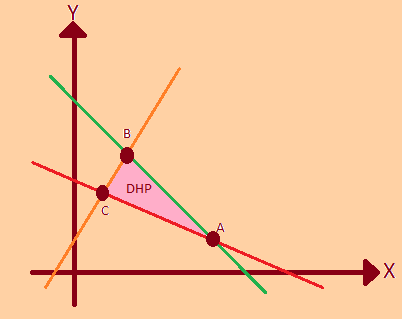
\includegraphics[scale=0.7]{dhp}
\caption{Daerah Hasil Penyelesaian (DHP)}
\end{figure}

Misalnya untuk gambar DHP di bawah ini kita bisa lihat bahwa titik pojok terdapat pada titik A, titik B, dan titik C.
\subsection{Contoh Soal}
\index{Examples!Contoh Soal}

\begin{example}
Tentukanlah nilai maksimum dan nilai minimum fungsi tujuan f(x,y) = 1500x + 1250y berdasarkan DHP berikut ini.
\begin{figure}[h]
\centering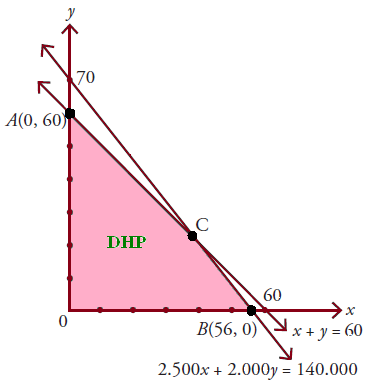
\includegraphics[scale=0.7]{contohsoaloptimum}
\end{figure}
\end{example}
Jawab:\\
Diketahui bahwa titik pojok yang terdapat pada gambar di atas adalah titik A,b,C dan O. Titik C belum mempunyai titik koordinat sehingga kita harus mencari terlebih dahulu dengan cara eliminasi kedua persamaan garis.\\
Menentukan titik C:
\begin{figure}[h]
\centering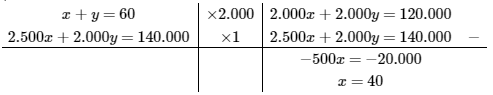
\includegraphics[scale=0.7]{eliminasi}
\end{figure}\\
Substitusi x=40 ke persamaan x + y = 60\\
x + y = 60\\
40 + y = 60\\
y = 20.\\
Sehingga titik C adalah C(40,20).\\
Substitusi semua titik pojok ke fungsi tujuan : f(x,y) = 1500x + 1250y.\\

\begin{tabular}{l l}
A(0,60) & f = 1500(0) + 1250(60) = 75000 \\
B(56,0) & f = 1500(56) + 1250(0) = 84000 \\
C(40,20) & f = 1500(40) + 1250(20) = 85000 \\
D(0,0) & f = 1500(0) + 1250(0) = 0 \\
\end{tabular}

Jadi fungsi f(x,y) = 1500x + 1250y di titik C(40,20) dengan nilai maksimumnya adalah f = 85000. Sedangkan untuk titik minimum f(x,y) = 1500x + 1250y di titik C(0,0) dengan nilai minimumnya adalah f = 0.

\subsection{Soal Latihan }\index{Lists!Soal Latihan}


\begin{exercise}

\begin{enumerate}
\item Tentukan nilai maksimum f(x,y) = 3x + 4y pada himpunan penyelesaian sistem pertidaksamaan berikut: $x + 2y \le 10, 4x + 3y \le 24, x \ge 0, y \ge 0.$
\item Tentukan nilai maksimum dan nilai minimum dari fungsi objektif z = 2x + 3y yang memenuhi $x + y \le 7, x \ge 0$, dan $y \ge 0, x,y \in R.$
\item Tentuan nilai maksimum Z = 2x + 5y dari daerah penyelesaian (daerah yang diarsir) pada gambar di bawah ini:\\
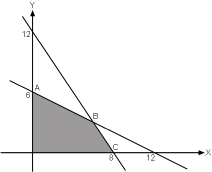
\includegraphics[scale=0.7]{soaloptimum}
\end{enumerate}
\end{exercise}

\section{Penerapan Program Linier Dua Variabel}\index{Penerapan Program Linier Dua Variabel}
Program linear banyak digunakan dalam kehidupan sehari-hari, misalnya dalam bidang ekonomi, perdagangan, dan pertanian.\\

Misalkan dalam bidang perdagangan atau pengusaha, para pedagang atau pengusaha tentu ingin memperoleh keuntungan maksimum. Sebelum melakukan transaksi ataupun pengambilan keputusan dalam usahanya, mereka pasti membuat perhitungan yang matang tentang langkah apa yang harus dilakukan. Oleh karena itu, diperlukan metode yang tepat dalam pengambilan keputusan pedagang atau pengusaha tersebut untuk memperoleh keuntungan maksimum dan meminimumkan kerugian yang mungkin terjadi.\\

Adapun untuk contoh penerapan lain misalkan sebagai berikut:
\begin{itemize}
\item Penerapan dalam Dunia Kerja\\
Dalam dunia kerja, matematika telah digunakan sebagai salah satu alat penyaring atau seleksi bagi orang untuk memperoleh pekerjaan yang lebih baik dengan gaji yang lebih tinggi. Juga tidak sedikit yang melibatkan penggunaan matematika atau proses berpikir matematis, misalnya melakukan jual-beli, mengukur luas tanah pekarangan, areal sawah, menimbang beras,gula, dan sembako lainnya, menghitung pengeluaran kebutuhan rumah tangga, menghitung biaya pembayaran rekening listrik dan PDAM, membayar hutang, dan sebagainya.

\item Penerapan dalam Dunia Rumah Tangga\\
Suatu saat ketika anda sudah menjadi seorang ibu rumah tangga, yang mengharuskan anda untuk terampil dalam mengelola keuangan rumah tangga, maka anda tidak akan lepas dari penggunaan ilmu matematika terutam bab aljabar. Mulai dari menganalisa pemasukan, mengatur pengeluaran untuk kebutuhan rumah tangga, uang saku anak, tabungan, sampai ke asuransi kesehatan.

\item Penerapan dalam Bidang Perdagangan\\
Dalam hal perdagangan, ambilah contoh yang paling sederhana, menjual buah-buahan, anda akan dituntut untuk punya kemampuan menganalisis laba rugi, berapa jumlah biaya yang harus dikeluarkan untuk "kulakan", berapa laba tiap kilogram buah dan buah apa saja yang memberi keuntungan maksimum. semua itu sedikit banyak akan menggunakan ilmu matematika khususnya program linier.
\end{itemize}
 
Seperti yang telah disinggungkan pada section sebelumnya, ada beberapa metode untuk menyelesaikan masalah program linear dua variabel, di antaranya yang kita bahas adalah metode uji titik pojok. Nah untuk contoh soal yang diambil dari kehidupan sehari-hari sebagai berikut:\\
\\
\begin{example}
Ling ling membeli 240 ton beras untuk dijual lagi. Ia menyewa dua jenis truk untuk mengangkut beras tersebut. Truk jenis A memiliki kapasitas 6 ton dan truk jenis B memiliki kapasitas 4 ton. Sewa tiap truk jenis A adalah Rp 100.000,00 sekali jalan dan truk jenis B adalah Rp 50.000,00 sekali jalan. Maka Ling ling menyewa truk itu sekurang-kurangnya 48 buah. Berapa banyak jenis truk A dan B yang harus disewa agar biaya yang
dikeluarkan minimum?
\end{example}
Jawab:\\
Untuk menyelesaikan masalah ini kita akan menggunakan metode uji titik sudut yang telah kita pelajari pada section nilai optimum fungsi objektif.\\
Dari soal di atas dapat diperoleh bahwa:
\begin{figure}[h]
\centering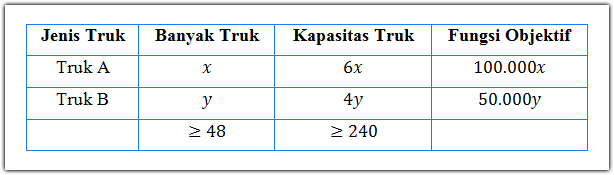
\includegraphics[scale=0.7]{jawab1}
\end{figure}\\
Dan ketika kita ubah ke model matematika akan seperti berikut:\\
$x + y \ge 48,$\\
$6x + 4y \ge 240,$\\
$x \ge 0, y \ge 0,$ x, y anggota bilangan cacah\\
\\
Dengan fungsi objektifnya yaitu  f(x, y) = 100.000x + 50.000y.\\
\begin{figure}[h]
\centering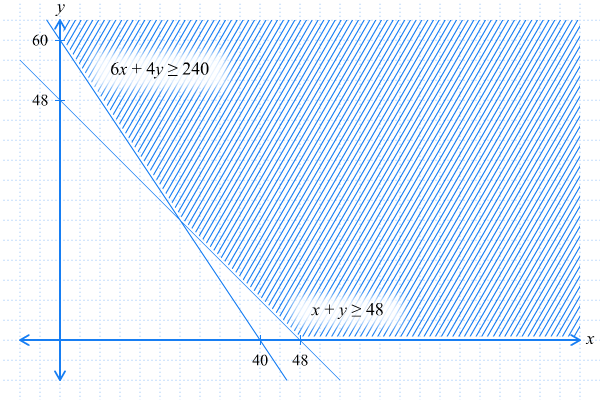
\includegraphics[scale=0.6]{jawab2}
\end{figure}\\
Dari gambar di atas dapat kita ketahui bahwa titik  pojok dari daerah penyelesaian di atas adalah titik potong garis 6x + 4y = 240 dengan sumbu-y, titik potong garis x + y = 48 dengan sumbu-x, dan titik potong garis-garis x + y = 48 dan 6x + 4y = 240.\\
Titik potong garis 6x + 4y = 240 dengan sumbu-y adalah titik (0, 60). Titik potong garis x + y = 48 dengan sumbu-x adalah titik (48, 0). Sedangkan titik potong garis-garis x + y = 48 dan 6x + 4y = 240 dapat dicari dengan menggunakan cara eliminasi berikut ini.\\
\begin{figure}[h]
\centering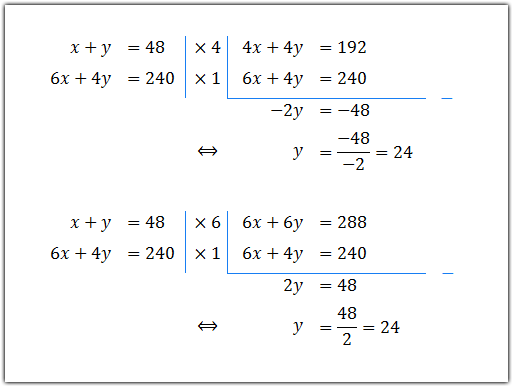
\includegraphics[scale=0.7]{jawab3}
\end{figure}\\

Substitusi semua titik pojok ke fungsi tujuan : f(x,y) = 100000x + 50000y.\\

\begin{tabular}{l l}
A(0,60) & f = 1500(0) + 1250(60) = 3000000 \\
B(48,0) & f = 1500(48) + 1250(0) = 4800000 \\
C(24,24) & f = 1500(24) + 1250(24) = 3600000 \\
D(0,0) & f = 1500(0) + 1250(0) = 0 \\
\end{tabular}


Jadi Dari ketiga hasil tersebut, dapat diperoleh bahwa agar biaya yang dikeluarkan minimum, Ling ling harus menyewa 60 truk jenis B dan tidak menyewa truk jenis A.\\

\begin{example}
Seorang pedagang menjual buah mangga dan pisang dengan menggunaknan gerobak. Pedagang tersebut membeli magga dengan harga Rp.8.000,00/kg dan pisang Rp.6000,00/kg. Modal yang tersedia Rp. 1.200.000,00 dan gerobaknya hanya dapat menampung mangga dan pisang sebanyak 180 kg. jika harga jual mangga Rp.9.200,00/kg dan pisang Rp.7000,00/kg, maka tentukanlah laba maksimum yang diperoleh pedagang tersebut!\\
\end{example}

Jawab:\\
Karena ditanya laba maksimum, maka fungsi tujuan/fungsi objektifnya adalah keuntungan dari menjual buah mangga dan buah pisang perkilonya.\\
Berikut untuk penjualan:\\
mangga = 9200 - 8000 = 1200\\
pisang = 7000 - 6000 = 1000\\

misalkan:\\
mangga = x\\
pisang = y\\

maka fungsi objektifnya adalah:\\
f(x,y)=1200x + 1000y\\

Model matematika atau sistem pertidaksamaan yang memenuhi soal tersebut adalah:\\
x + y <= 180\\
8000x + 6000y <= 1200000 --> 4x + 3y <=600\\
x>=0\\
y>=0\\

Titik potong masing-masing garis terhadap sumbu x dan sumbuy:\\
Garis x + y = 180\\
untuk x = 0, y = 180 --> (0,180)\\
untuk y = 0, x = 180 --> (180,0)\\

Garis 4x + 3y = 600\\
untuk x = 0, y = 200 --> (0,200)\\
untuk y = 0, x = 150 --> (150,0)\\

Himpunan penyelesaian sistem pertidaksamaan adalah:\\
\begin{figure}[h]
\centering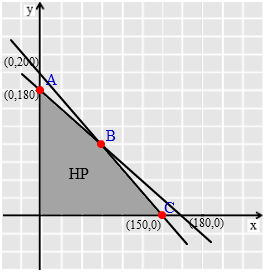
\includegraphics[scale=0.99]{jawabA}
\end{figure}\\
Dari grafik diketahui ada tiga titik pojok yaitu A, B dan C. Titik C merupakan perpotongan antara garis x + y = 180 dengan 4x + 3y = 600.\\
x  +  y = 180 | x3 | 3x + 3y = 540\\
4x + 3y = 600 | x1 | 4x + 3y = 600 dikurangi.\\
maka -x = -60 maka x = 60.\\

Maka x tersebut dimasukan ke dalam persamaan x + y = 180.\\

x + y = 180\\
y = 180-60\\
y = 120\\

Kemudian substitusikan titik pojok pada fungsi objektif f(x,y) 1200x + 1000y:\\
\begin{tabular}{l l}
A(0,180) & f = 1000(180) = 180000 \\
B(60,120) & f = 1200(60) + 1000(120) = 192000 \\
C(150,0) & f = 1200(150)= 180000 \\
D(0,0) & f = 1500(0) + 1250(0) = 0 \\
\end{tabular}

Jadi laba maksimum yang diperoleh pedagang buah adalah Rp.192.000,00


\subsection{Soal Latihan Penerapan Program Linear Dua Variabel}\index{Lists!Soal Latihan Penerapan Program Linear Dua Variabel}


\begin{exercise}

\begin{enumerate}
\item Seorang pembuat kue mempunyai 8 kg tepung dan 2 kg gula pasir. Ia ingin membuat dua macam kue yaitu kue dadar dan kue apem. Untuk membuat kue dadar dibutuhkan 10gram gula pasir dan 20 gram tepung sedangkan untuk membuat sebuahkue apem dibutuhkan 5 gram gula pasir dan 50 gram tepung. Jika kue dadar dijual dengan harga Rp.300,00/buah dan kue apem dijual dengan harga Rp. 500,00/buah, tentukanlah pendapatan maksimum yang dapat diperoleh pembuat kue tersebut!
\item Menjelang hari raya Idul Adha, Pak Mahmud hendak menjual sapi dan kerbau. Harga seekor sapi dan kerbau di Medan berturut-turut Rp.9.000.000,00 dan Rp.8.000.000,00. Modal yang dimiliki pak Mahmud adalah Rp.124.000.000,00. Pak Mahmud menjual sapi dan kerbau di Aceh dengan harga berturut-turut Rp.10.300.000,00 dan Rp.9.200.000,00. Kandang yang ia miliki hanya dapat menampung tidak lebih dari 15 ekor. Agar mencapai keuntungan maksimum, tentukanlah banyak sapi dan kerbau yang harus dibeli pak Mahmud!
\end{enumerate}
\end{exercise}

%----------------------------------------------------------------------------------------
%	CHAPTER 5
%----------------------------------------------------------------------------------------

\chapterimage{chapter_head_2.pdf} % Chapter heading image

\chapter{Matriks}

\section{Pengertian Matriks}\index{Pengertian Matriks}

\section{Operasi Matriks}\index{Operasi Matriks}

\section{Determinan dan Invers Matriks Berorde 2x2 dan 3x3 }\index{Determinan dan Invers Matriks Berorde 2x2 dan 3x3 }

\section{Pemakaian Matriks Pada Pransformasi Geometri}\index{Pemakaian Matriks Pada Pransformasi Geometri}

\begin{center}
\LARGE \textbf{Pemakaian Matriks pada Transformasi Geometri}
\end{center}

\begin{enumerate}
\item \textbf{Apa itu Transformasi Geometri?}

\begin{enumerate}
\item \textbf{ Pengertian Transformasi Geometri?}
\end{enumerate}
\end{enumerate}

\noindent 
 Pengertian transformasi geometri adalah proses mengubah setiap titik koordinat menjadi titik koordinat lain pada bidang tertentu. Transformasi bisa juga dilakukan pada kumpulan titik yang membentuk bidang/bangun tertentu. Jika sobat punya sebuah titik A (x,y) kemudian ditransformasikan oleh transformasi T maka akan menghasilkan titik yang baru A’ (x’,y’). Secara matematis di tulis:

\noindent 
\noindent 
\noindent 
\begin{center}
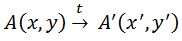
\includegraphics{Pictures/1.PNG}\\
\end{center}

\begin{enumerate}
	\item \textbf{Jenis-Jenis Transformasi Geometri}
\end{enumerate}

\noindent 
Sebuah objek dapat diubah dengan melakukan berbagai perlakuan. Di dalam transformasi geometri dikenal adanya 4 jenis transformasi yang bisa dilakukan terdapat sebuah koordinat yaitu menggesernya, mencerminkannya, memutar, memperbesar, atau mengecilkan. Selain 4 transformasi tersebut masih ada yang namanya regangan dan gusuran. Yuk lihat ulasannya satu persatu di bawah ini.

\noindent 
\begin{center}
	\noindent \includegraphics*[width=2.32in, height=1.48in, keepaspectratio=false, trim=0.00in 0.11in 0.00in 0.00in]{Pictures/2.PNG}
\end{center}
\noindent 
\noindent \textbf{a. Translasi (Pergeseran)}
\noindent 
Translasi atau pergeseran adalah transformasi yang memindahkan setiap titik pada bidang menurut jarak dan arah tertentu. Sobat bisa mengatakan kalau translasi hanya memindahkan tanpa mengubah ukuran tanpa memutar. Kata kuncinya transformasik ke arah yang sama dan ke jarak yang sama. Misalkan sobat punya sebuah titik T (x,y)  yang ditranslasikan menurut (a,b) maka hasil setelah transfromasi  adalah:

\noindent 
\begin{center}
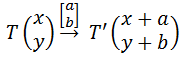
\includegraphics{Pictures/3.PNG}\\
\end{center}

\noindent (x’,y’) = (x+a, y+b)
\noindent 

\noindent Relasi antara anggota himpunan A ke himpunan B yang mungkin adalah menyukasi atau menyenangi.

\noindent Dari contoh di atas, himpunan A tersebut domain (daerah asal) dan himpunan B disebut daerah tujuan (ko-domain) . Sementara itu menyukasi disebut relasi. Himpunan semua anggota ko-domain di sebut range (daerah hasil).

\noindent 

\noindent \textbf{b. Refleksi}

\noindent 

Refleksi atau sering disebut dengan istilah pencerminan adalah suatu transformasi dengan memindahkan setiap titik pada bidang dengan menggunakan sifat-sifat pencerminan pada cermin datar. Berikut tabel transformasi pencerminan:


\begin{center}
	\noindent \includegraphics*[width=2.32in, height=1.48in, keepaspectratio=false, trim=0.00in 0.11in 0.00in 0.00in]{Pictures/4.PNG}
\end{center}

\newpage
\noindent \textbf{c. rotasi}

\begin{center}
	\noindent \includegraphics*[width=2.32in, height=1.48in, keepaspectratio=false, trim=0.00in 0.11in 0.00in 0.00in]{Pictures/5.PNG}
\end{center}
\noindent 
Rotasi adalah memutar setiap titik pada bidang dengan menggunakan titik pusat tertentuk yang memiliki jarak sama dengan setiap titik yang diputar (jari-jari). Rotasi tidak mengubah ukuran benda sama sekali. Ada dua macam rotasi, rotasi dengan titik pusat (0,0) dan rotasi dengan titik tertentu P (a,b).

\noindent \textbf{1. Rotasi dengan Titik Pusat (0,0) dengan Sudut Putar $\alpha$}
\begin{center}
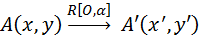
\includegraphics{Pictures/6.PNG}\\
\end{center}

\noindent
dimana

\noindent x’ = x cos $\alpha$ – y sin
\noindent y’ = x sin $\alpha$ + y cos $\alpha$

atau jika dibuat matriks transformasinya menjadi

\noindent
\begin{center}
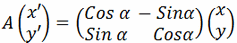
\includegraphics{Pictures/7.PNG}\\
\end{center}

\noindent
keterangan

\noindent $\alpha$  bernilai + jika arah putaran berlawanan dengan arah jarum jam
\noindent $\alpha$ bernilai – jika araha putaran searah dengan arah jarum jam


\noindent \textbf{2.Rotasi dengan Titik Pusat (a,b) dengan Sudut Putar $\alpha$}

\noindent
Jika sobat punya sebuah titik (x,y) yang diputar sebesar $\alpha$ derajat dengant titik pusat P (a,b) maka:
\noindent
\begin{center}
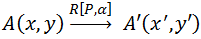
\includegraphics{Pictures/8.PNG}\\
\end{center}


\noindent
dimana
\noindent x’ – a = (x-a) cos $\alpha$ – (y-b) sin $\alpha$
\noindent y’ – b = (x-a) sin $\alpha$  + (y-b) cos $\alpha$

\noindent \textbf{d. Dilatasi (Perkalian)}

\noindent
\begin{center}
	\noindent \includegraphics*[width=2.32in, height=1.48in, keepaspectratio=false, trim=0.00in 0.11in 0.00in 0.00in]{Pictures/9.PNG}
\end{center}

\noindent
Selain dipindah, dicerminkan, dan diputar, transformasi juga bisa berbentuk pembesaran atau pengecilan yang disebut dilatasi. Faktor yang menyebabkan diperbesar atau diperkecilnya suatu bangun dinamakan faktor dilatasi. Faktor dilatis dilambangkan dengan k dimana


\noindent Jika k > 1 atau k <-1 maka diperbesar
\noindent Jika -1 < k < 1 maka diperkecil
\noindent Jika k = 1 atau k = -1 maka bangun tidak mengalami perubahan ukuran

\noindent 1. Dilatasi terhadap titik pusat O (0,0)Dilatasi dengan pusat O (0,0) dan faktor dilatasi K maka
\noindent
\begin{center}
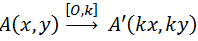
\includegraphics{Pictures/10.PNG}\\
\end{center}

\noindent
\begin{center}
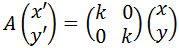
\includegraphics{Pictures/11.PNG}\\
\end{center}

\noindent
2. Dilatasi terhadap titik pusat P (a,b)Jika sebuah titik didilatasi dengan faktor dilatasi k dan titik pust P (a,b) maka
\noindent
\begin{center}
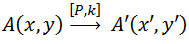
\includegraphics{Pictures/12.PNG}\\
\end{center}

\noindent
\begin{center}
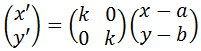
\includegraphics{Pictures/13.PNG}\\
\end{center}

\noindent
\noindent dimana
\noindent x’-a = k (x-a)
\noindent y’-b = k (y-b)

\noindent \textbf{e. Gusuran (Shearing)}
\noindent Gusuran artinya menggeser serah sumbu x atau sumbu y dengan faktor skala tertentu. Coba sobat perhatikan gambar di bawah ini:

\noindent
\begin{center}
	\noindent \includegraphics*[width=2.32in, height=1.48in, keepaspectratio=false, trim=0.00in 0.11in 0.00in 0.00in]{Pictures/14.PNG}
\end{center}
\noindent 
Segi empat di atas dapat di gusur menurut sumbu x atau sumbu y dengan skala gusur k

\noindent
\noindent Untuk gusuran menurut sumbu x —> Jika nilai k positif maka ke kanan, k negatif maka ke kiri
\noindent Untuk gusuran menurut sumbu y —> Jika nilai k positif maka ke atas, k kengatif maka k bawah

\noindent
Dari penjelasan di atas maka dapat disimpulkan rumus:
\noindent
\begin{center}
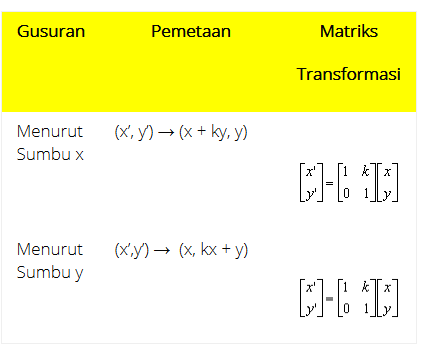
\includegraphics{Pictures/15.PNG}\\
\end{center}
\noindent \textbf{e. Gusuran (Shearing)}
\noindent
\begin{center}
	\noindent \includegraphics*[width=2.32in, height=1.48in, keepaspectratio=false, trim=0.00in 0.11in 0.00in 0.00in]{Pictures/16.PNG}
\end{center}

\noindent
Regangan atau dalam bahasa inggris disebut streching  artinya transformasi dengan menarik sebuah benda searah sumbu x atau sumbu y dengan skala tertentu. Jika sobat punya sebuah titik (x,y) yang ditari ke arah sumbu x atau y dengan skala k maka hasil pemetaannya dapat dicari dengan rumus
\noindent
\begin{center}
	\noindent \includegraphics*[width=2.32in, height=1.48in, keepaspectratio=false, trim=0.00in 0.11in 0.00in 0.00in]{Pictures/17.PNG}
\end{center}

\noindent

\begin{enumerate}
	\item  \textbf{Komposisi Transformasi}
\end{enumerate}
\noindent
Komposisi transformasi adalah gabungan dari dua atau lebih transformasi baik berbeda ataupun sama.  Misalkan sebuah titik di transformasikan 2 kali oleh T1 dan T2 maka secara matematis dituliskan T1o T2 dengan matriks komposisi tersebut adalah perkalian dari matriks transformasi 2 dengan matriks transformasi 1 (dibalik).

\noindent
\begin{center}
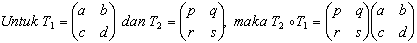
\includegraphics{Pictures/18.PNG}\\
\end{center}
\noindent
\begin{enumerate}
	\item  \textbf{Matriks Transformasi Khusus}
\end{enumerate}
\noindent
Berikut kami rangkumkan matriks tansformasi yang sering digunakan dalam soal-soal. Matriks di bawah ini juga akan memudahkan sobat untuk mencari matriks dari komposisi dua atau lebih transformasi.

\noindent
\begin{center}
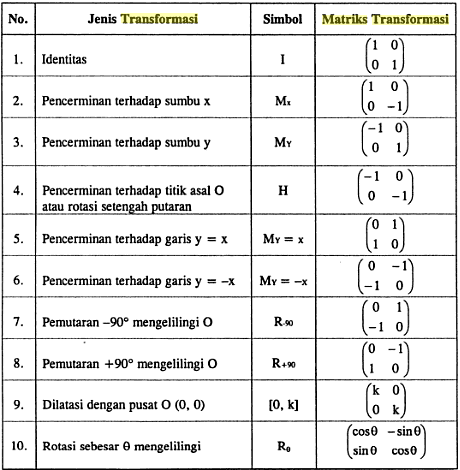
\includegraphics{Pictures/19.PNG}\\
\end{center}

\textbf{Contoh Soal 1}
\noindent Titik A(5,-2) ditranslasi oleh  T (-3, 1). Tentukan koordinat bayangan titik A tersebut!\\

A. A’(2,1)\\

B. A’(1,1)\\

C. A’(2,2)\\

D. A’(2,-1)\\

E. A’(-2,1)\\

Pembahasan :

\noindent
\begin{center}
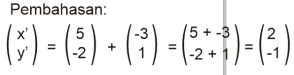
\includegraphics{Pictures/28.jpg}\\
\end{center}

\textbf{Contoh Soal 2}
\noindent Tentukan bayangan garis y = 3x – 5 oleh translasi T (-2, 1)!

A. y = 2x + 2\\

B. y = 2x – 2\\

C. y = 3x + 2\\

D. y = 3x – 2\\

E. y = 2x + 3\\

\noindent
\begin{center}
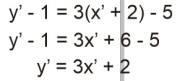
\includegraphics{Pictures/29.jpg}\\
\end{center}

\textbf{Contoh Soal 3}
\noindent Tentukan bayangan titik (5, -3) oleh rotasi R(P, 90) dengan koordinat titik P(-1, 2)!

A. (8, 4)\\

B. (-8, 4)\\

C. (8, -4)\\

D. (-4,- 8)\\

E. (4, 8)\\

Pembahasan :\\

\noindent
\begin{center}
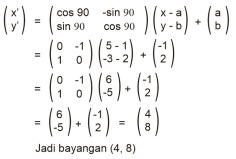
\includegraphics{Pictures/30.jpg}\\
\end{center}
 \textbf{Contoh Soal 4}
\noindent Tentukan bayangan titik (9, 3) oleh dilatasi [O, 1/3]!

A. (1, 3)\\

B. (3, 1)\\

C. (-1, -3)\\

D. (3, -1)\\

E. (1, -3)\\

Pembahasan:\\

\noindent
\begin{center}
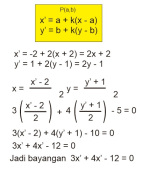
\includegraphics{Pictures/31.jpg}\\
\end{center}

 \textbf{Contoh Soal 5}
\noindent Tentukan bayangan garis 3x + 4y – 5 = 0 oleh dilatasi dengan pusat (-2, 1) dan faktor skala 2!

A. 3x + 4y + 12 = 0 \\

B. 3x + 4y – 12 = 0 \\

C. 3x – 4y + 12 = 0\\

D. -3x + 4y + 12 = 0\\

E. 3x – 4y – 12 = 0\\

Pembahasan :\\

\noindent
\begin{center}
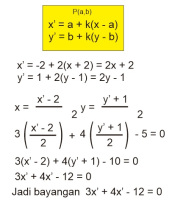
\includegraphics{Pictures/32.jpg}\\
\end{center} 

%----------------------------------------------------------------------------------------
%	CHAPTER 6
%----------------------------------------------------------------------------------------

\chapterimage{chapter_head_2.pdf} % Chapter heading image

\chapter{Barisan dan Deret}

\section{Pola Bilangan}\index{Pola Bilangan}
\begin{center}
	\LARGE \textbf{Pola Bilangan}
\end{center}
\noindent
Berawal dari tugas matematika di sekolah oleh guru matemtika yang memberi tugas untuk mencari pola – pola bilangan matematika, maka pada kesempatan kali ini saya akan membagikan beberapa jenis pola bilangan matematika. Tanpa panjang lebar, langsung saja kita ke pembahasannya.\\
\noindent
\begin{enumerate}
	\item  \textbf{Pola bilangan ganjil}
\end{enumerate}
\noindent
\begin{center}
	\noindent \includegraphics*[width=2.32in, height=1.48in, keepaspectratio=false, trim=0.00in 0.11in 0.00in 0.00in]{Pictures/21.PNG}
\end{center}
\noindent
\noindent Pola bilangan ganjil memiliki pola 1, 3, 5, 7, 9 ….\\
\noindent bilangan ganjil adalah 1,3, 5, 7, 9, …\\
\noindent Deret bilangan ganjil adalah 1 + 3 + 5 + 7 + 9 + ….\\
\noindent Rumus mencari suku ke ke-n adalah Un = 2n – 1\\
\noindent Rumus mencari jumlah n suku pertama adalah Sn = n2\\
\noindent Berikut adalah gambar pola dari bilangan ganjil\\

\noindent
\begin{enumerate}
	\item  \textbf{ Pola bilangan genap}
\end{enumerate}
\noindent
\begin{center}
	\noindent \includegraphics*[width=2.32in, height=1.48in, keepaspectratio=false, trim=0.00in 0.11in 0.00in 0.00in]{Pictures/22.PNG}
\end{center}

\noindent
\noindent Pola bilangan genap adalah 2, 4, 6, 8, 10, …..\\
\noindent Barisan bilangan genap adalah 2, 4, 6, 8, 10, ….\\
\noindent bilangan genap adalah 2 + 4 + 6 + 8 + 10 + …..\\
\noindent Rumus untuk mencari suku ke-n adalah Un = 2n\\
\noindent Rumus mencari jumlah n suku pertama adalah Sn = n2 + n\\
\noindent Gambar pola bilangan genap adalah sebagai berikut\\
\begin{enumerate}
	\item  \textbf{  Pola bilangan segitiga}
\end{enumerate}
\noindent
\begin{center}
	\noindent \includegraphics*[width=2.32in, height=1.48in, keepaspectratio=false, trim=0.00in 0.11in 0.00in 0.00in]{Pictures/23.JPG}
\end{center}
\noindent
\noindent Pola bilangan segitiga adalah 1, 3, 6, 10, 15, 21, …..\\
\noindent Barisan bilangan segitiga adalah 1, 3, 6, 10, 15, 21, …..\\
\noindent Deret bilangan segitiga adalah 1 + 3 + 6 + 10 + 15 + 21 + …..\\
\noindent Rumus mencari suku ke-n adalah Un = 1/2 n (n + 1 ).\\
\noindent Rumus mencari jumlah n suku pertama adalah Sn = 1/6 n ( n + 1 ) ( n + 2 ).\\
\noindent Gambar pola bilangan segitiga adalah sebagai berikut.\\

\noindent
\begin{enumerate}
	\item  \textbf{ Pola bilangan Persegi}
\end{enumerate}
\noindent
\begin{center}
	\noindent \includegraphics*[width=2.32in, height=1.48in, keepaspectratio=false, trim=0.00in 0.11in 0.00in 0.00in]{Pictures/24.PNG}
\end{center}
\noindent
\noindent$\bullet$  Pola bilangan persegi adalah 1, 4, 9, 16, 25, …..\\
\noindent $\bullet$ Barisan bilangan persegi adalah 1, 4, 9, 16, 25, …..\\
\noindent$\bullet$ Deret bilangan persegi adalah 1 + 4 + 9 + 16 + 25 + …….\\
\noindent$\bullet$ Rumus mencari suku ke-n adalah Un = n2.\\
\noindent $\bullet$ Rumus mencari jumlah n suku pertama adalah Sn = 1/6 n ( n + 1 ) ( 2n + 1 ).\\
\noindent $\bullet$ Gambar pola bilangan persegi adalah sebagai berikut.\\

\noindent
\begin{enumerate}
	\item  \textbf{ Pola bilangan persegi panjang}
\end{enumerate}
\noindent
\begin{center}
	\noindent \includegraphics*[width=2.32in, height=1.48in, keepaspectratio=false, trim=0.00in 0.11in 0.00in 0.00in]{Pictures/25.PNG}
\end{center}
\noindent
\noindent  $\bullet$ Pola bilangan persegi panjang adalah 2, 6, 12, 20, 30, …….\\
\noindent  $\bullet$ Barisan bilangan persegi panjang adalah 2, 6, 12, 20, 30, …….\\
\noindent $\bullet$  Deret bilangan persegi panjang adalah 2 + 6 + 12 + 20 + 30 + …..\\
\noindent  $\bullet$ Rumus mencari suku ke-n adalah Un = n ( n + 1 ).\\
\noindent $\bullet$  Rumus mencari jumlah n suku pertama adalah Sn = 1/3 n ( n + 1 ) ( n + 2 ).\\
\noindent $\bullet$  Gambar pola bilangan persegi panjang adalah sebagai berikut.\\
\noindent
\begin{enumerate}
	\item  \textbf{ Pola bilangan segitiga pascal}
\end{enumerate}
\noindent
\begin{center}
	\noindent \includegraphics*[width=2.32in, height=1.48in, keepaspectratio=false, trim=0.00in 0.11in 0.00in 0.00in]{Pictures/26.PNG}
\end{center}
\noindent
\noindent Rumus mencari jumlah baris ke-n adalah 2n – 1
\\
\begin{enumerate}
	\item  \textbf{  Pola bilangan Fibonacci}
\end{enumerate}

\noindent $\bullet$ Pola bilangan fibanocci adalah pola bilangan dimana jumlah bilangan setelahnya merupakan hasil dari penjumlahan dari dua bilangan sebelumnya.\\
\noindent$\bullet$ Pola bilangan Fibonacci adalah 1, 1, 2, 3, 5, 8, 13, 21, 34, …..\\
\noindent $\bullet$ 2 diperoleh dari hasil 1 + 1 3 diperoleh dari hasil 2 + 1, 5 diperoleh dari hasil 3 + 2 dan seterusnya.\\
\noindent  $\bullet$ Rumus mencari suku ke-n adalah Un = Un – 1 + Un - 2.\\

\noindent
\begin{enumerate}
	\item  \textbf{  Pola bilangan pangkat tiga}
\end{enumerate}
\noindent
\noindent $\bullet$ Pola bilangan pangkat tiga adalah pola bilangan dimana bilangan setelahnya merupakan hasil dari pangkat tiga dari bilangan sebelumnya.\\
\noindent $\bullet$ Contoh pola bilangan pangkat tiga adalah 2, 8, 512, 134217728, …..\\
\noindent  $\bullet$ Keterangan : 8 diperoleh dari hasil 2 pangkat tiga, 512 diperoleh dari hasil 8 pangkat tiga, dan seterusnya.\\

\noindent
\begin{enumerate}
	\item  \textbf{  Pola bilangan aritmatika}
\end{enumerate}
\noindent
\noindent$\bullet$ Pola bilangan aritmatika adalah pola bilangan dimana bilangan sebelum dan sesudahnya memiliki selisih yang sama.\\
\noindent $\bullet$ Contoh pola bilangan aritmatika adalah 2, 5, 8, 11, 14, 17, ….\\
\noindent $\bullet$ Suku pertama dalam bilangan aritmatika dapat disebut dengan awal ( a ) atau U1, sedangkan suku kedua adalah U2 dan seterusnya.\\
\noindent $\bullet$ Selisih dalam barisan aritmatika disebut dengan beda dan dilambangkan dengan b.\\
\noindent $\bullet$ Karena bilangan sebelum dan sesudahnya memiliki selisih yang sama, maka b = U2 - U1 = U3 – U2 = U4 – U3 = U5 – U4 = U6 – U5 = 3.\\
\noindent $\bullet$ Rumus mencari suku ke-n adalah Un = a + ( n – 1 ) b.\\
\noindent $\bullet$ Rumus mencari jumlah n suku pertama adalah Sn = n/2 ( a + Un ) atau Sn = n/2 ( 2 a + ( n – 1 ) b ).\\
\noindent

\textbf {Contoh soal :} 
\noindent Tentukanlah jumlah 7 bilangan asli ganjil yang pertama !\\

\textbf {jawab :}
\noindent ketujuh bilangan tersebut adalah : 1, 3, 5, 7, 9, 11, 13. jadi n=7\\
\noindent $\blacktriangleright$ jumlah ke-7 bilangan tersebut adalah 72=49\\
\noindent $\blacktriangleright$ untuk membuktikan silahkan dihitung manual 1+3+5+7+9+11+13=...?\\

\textbf {Contoh 2 pola bilangan}
\noindent Berapakah banya bilangan asli ganjil yang jumlahnya 81 ?\\

\textbf {jawab :}
\noindent Kita telah mengetahui bahwa jumlah bilangan asli ganjil yaitu banyaknya bilangan asli ganjil dikuadratkan secara sederhana dapat kita tuliskan n2 dari pertanyaan diatas dapat kita simpulkan bahwa
n2=81, maka\\
n = $\surd$81\\
n = 9, jadi banyaknya bilangan ganjil adalah 9.\\

\textbf {Contoh Soal Pola Bilangan Genap}
\noindent Selain bilangan ganjil, bilangan genap juga termasuk anggota dari bilangan asli yaitu {2, 4, 6, 8, ...}\\

Perhatikan susunan heksagonal seperti pada gambar berikut :\\
\noindent
\begin{center}
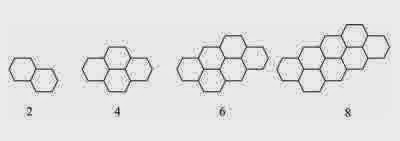
\includegraphics{Pictures/27.jpg}\\
\end{center}

\noindent pola bilangan matematika - pola heksagonal\\
\noindent  Gambar diatas menunjukkan bahwa heksagonal yang terdiri sebanyak bilangan genap dapat disusun membentuk pola tertentu. sehingga gambar diatas bisa disebut sebagai pola bilangan genap.\\

\noindent Untuk lebih memahami perhatikan uraian penjumlahan bilangan asli genap berikut :\\
Penjumlahan dari 2 bilangan genap :
2 + 4 = 6, n=2 dapat ditulis 6 = 2 (2+1)\\
penjumlahan 3 bilangan genap :
2 + 4 + 6 = 12, n=3 dapat ditulis 12 = 3 ( 3+1)\\
penjulahan 4 bilangan genap :
2 + 4 + 6 + 8 = 20, n=4 dapat ditulis 20 = 4 (4+1)\\

dari pola di atas seharusnya anda sudah dapat menarik kesimpulan rumus jumlah pola bilangan genap, ya benar rumusnya adalah ns = n ( n + 1 )\\


\section{Barisan dan Deret Aritmatika}\index{Barisan dan Deret Aritmatika}
Pengertian Barisan Aritmatika
Sebelum memahami pengertian barisan aritmatika kita harus mengetahui terlebih dahulumengenai pengertian basiran bilangan. Barisan bilangan merupakan sebuah urutan dari bilangan yang dibentuk dengan berdasarkan kepada aturan-aturan tertentu. Edangkan barisan aritmetika dapat didefinisikan sebagai suatu barisan bilangan yang tiap-tiap pasangan suku yang berurutan mengandung nilai selisih yang sama persis, contohnya adalah barisan bilangan: 2, 4 , 6, 8, 10, 12, 14, …

Barisan bilangan tersebut dapat disebut sebagai barisana aritmatika karena masing-masing suku memiliki selisih yang sama yaitu 2. Nilai selisih yang muncul pada barisan aritmatika biasa dilambangkan dengan menggunakan huruf b. Setiap bilangan yang membentuk urutan suatu barisan aritmatika disebut dengan suku. Suku ke n dari sebuah barisan aritmatika dapat disimbolkan dengan lambang Un jadi untuk menuliskan suku ke 3 dari sebuah barisan kita dapat menulis U3. Namun, ada pengecualian khusus untuk suku pertama di dalam sebuah barisan bilangan, suku pertama disimbolkan dengan menggunakan huruf a.

Maka, secara umum suatu barian aritmatika memiliki bentuk :

U1,U2,U3,U4,U5,…Un-1
a, atb, a+2b, a+3b, a+4b,…a+(n-1)b

Cara Menentukan Rumus suku ke-n dari Sebuah Barisan
Pada barisan aritmatika, mencaru rumus suku ke-n menjadi lebih mudah karena memiliki nilai selisih yang sama, sehingga rumusnya adalah:

U2 = a + b
U3 = u2 + b = (a + b) + b = a + 2b
U4 = u3 + b = (a + 2b) + b = a + 3b
U5 = u4 + b = (a + 3b) + b = a + 4b
U6 = u5 + b = (a + 4b) + b = a + 5b
U7 = u6 + b = (a + 5b) + b = a + 6b
.
\section{Barisan dan Deret Geometri}\index{Barisan dan Deret Geometri}
\textbf{Pengertian dan Rumus Geometri}

Barisan Geometri dapat didefinisikan sebagai barisan yang tiap-tiap sukunya didapatkan dari hasil perkalian suku sebelumnya dengan sebuah konstanta tertentu.

\textbf{Contoh Barisan Geometri}

 untuk lebih memahami apa yang dimaksud dengan barisan geometri perhatikan contoh berikut:
 
\textbf{3, 9, 27 , 81, 243, ...}

Barisan di atas adalah contoh barisan geometri dimana setiap suku pada barisan tersebut merupakan hasil dari perkalian suku sebelumnya dengan konstanta 3. maka bisa disimpulkan bahwa rasio pada barisan di atas adalah 3. rasio pada suatu barisan dapat dirumuskan menjadi:

\textbf{r = ak+1/ak}

Dimana ak adalah sembarang suku dari barisan geometri yang ada. sementara ak+1 adalah suku selanjutnya setelah ak.

Untuk menentukan suku ke-n dari sebuah barisan geometri, kita dapat menggunakan rumus:

\textbf{$Un = ar^n-1$}

\textbf{ Pengertian dan Rumus deret Geometri}

Deret geometri dapat diartikan sebagai jumlah dari n suku pertama pada sebuah barisan geometri. apabila suku ke-n dari suatu barisan geometri digambarkan dengan rumus: an = a1rn-1, maka deret geometrinya dapat dijabarkan menjadi:

\textbf{$Sn = a1 + a1r + a1r^2 + a1r^3 + ... + a1r^n-1$}

Apabila kita mengalikan deret geometri di atas dengan -r, lalu kita jumlahkan hasilnya dengan deret aslinya, maka kita akan memperoleh:

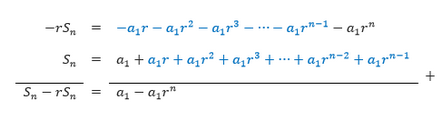
\includegraphics[width = 10cm, height= 4cm]{geometri1.png} 

%----------------------------------------------------------------------------------------
%	PART
%----------------------------------------------------------------------------------------

\part{Part Two}

%----------------------------------------------------------------------------------------
%	CHAPTER 7
%----------------------------------------------------------------------------------------

\chapterimage{chapter_head_1.pdf} % Chapter heading image

\chapter{Limit Fungsi Aljabar}

\section{Table}\index{Table}

\begin{table}[h]
\centering
\begin{tabular}{l l l}
\toprule
\textbf{Treatments} & \textbf{Response 1} & \textbf{Response 2}\\
\midrule
Treatment 1 & 0.0003262 & 0.562 \\
Treatment 2 & 0.0015681 & 0.910 \\
Treatment 3 & 0.0009271 & 0.296 \\
\bottomrule
\end{tabular}
\caption{Table caption}
\end{table}

%------------------------------------------------

\section{Figure}\index{Figure}

\begin{figure}[h]
\centering
\includegraphics[scale=0.5]{placeholder}
\caption{Figure caption}
\end{figure}

%----------------------------------------------------------------------------------------
%	CHAPTER 8
%----------------------------------------------------------------------------------------

\chapterimage{chapter_head_2.pdf} % Chapter heading image

\chapter{Turunan Fungsi Aljabar}

\section{Pengertian Turunan}\index{Pengertian Turunan}
\begin{center}
\LARGE \textbf{Turunan}
\end{center}

\noindent
Secara umum turunan banyak digunakan dalam kehidupan sehari-hari atau dalam bidang ilmu lainnya. Karena setiap bidang ilmu pasti saling terkait atau saling membutuhkan. Kegunaan yang sering kita ketahui itu menghitung garis singgung suatu kurva atau fungsi dan kecepatan sesaat. Selain itu juga digunakan untuk laju pertumbuhan organisme (biologi), keuntungan marjinal (ekonomi), kepadatan kawat (fisika) dan laju pemisahan (kimia). Kegunaan semua yang telah disebut diatas adalah memiliki konsep yang sama, yaitu konsep turunan.

\noindent
\begin{enumerate}
\item \textbf{Pengertian Turunan }
\end{enumerate}

\noindent 
Turunan merupakan salah satu dasar atau fundasi dalam analisis sehingga penguasaan kamu terhadap berbagai konsep dan prinsip turunan fungsi membantu kamu memecahkan suatu permasalahan dalam kehidupan sehari-hari. Suatu fungsi dapat dianalisis berdasarkan ide naik/turun, keoptimalan dan titik beloknya dengan menggunakan konsep turunan. Pada bagian berikut, kita akan mencoba mengamati berbagai permasalahan nyata dan mempelajari beberapa kasus dan contoh untuk menemukan konsep turunan. Kita memulainya dengan menemukan konsep persamaan garis tangen/singgung.

\noindent 
\begin{enumerate}
\item \textbf{Menemukan Konsep Garis Sekan dan Garis Tangen}
\end{enumerate}

\noindent 
Coba kamu amati dan cermati berbagai masalah nyata yang diajukan, bermanfaat sebagai sumber abstraksi kita dalam menemukan konsep dan hubungan antara garis sekan atau tali busur dan garis singgung.\\

\noindent 
\textbf{Masalah:}

\noindent 
Seorang pemain ski meluncur kencang di permukaan es yang bergelombang. Dia meluncur turun kemudian naik mengikuti lekukan permukaan es sehingga di suatu saat, dia melayang ke udara dan turun kembali ke permukaan. Perhatikan Gmbar di bawah ini.

\noindent
\begin{center}
\noindent \includegraphics*[width=1.90in, height=1.90in, keepaspectratio=false, trim=0.00in 0.11in 0.00in 0.00in]{Pictures/TurunanFungsi1.JPG}\\
\end{center}

\noindent 
Secara analitik, misalkan bahwa bukit es disketsa pada bidang (dimensi dua) dengan sudut pandang tegak lurus ke depan sehingga terdapat garis dan papan ski adalah sebuah garis lurus. Dapatkah kamu tunjukkan hubungan kedua garis tersebut?\\

\noindent 
\textbf{Alternatif Penyelesaian}

\noindent 
Coba kamu amati gambar di bawah ini. Misalkan deskripsi permasalahan di atas ditampilkan dalam bentuk gambar berikut. 

\noindent
\begin{center}
\noindent \includegraphics*[width=2.90in, height=2.19in, keepaspectratio=false, trim=0.00in 0.11in 0.00in 0.00in]{Pictures/TurunanFungsi2.JPG}
\end{center}

\noindent 
Posisi tegak pemain terhadap papan ski adalah sebuah garis yang disebut garis normal. Papan ski yang menyinggung permukaan bukit es di saat melayang ke udara adalah sebuah garis yang menyinggung kurva disebut garis singgung. Jadi, garis singgung tegak lurus dengan garis normal. Tujuan kita adalah mendapatkan persamaan garis singgung (PGS).

\noindent 
Misalkan pemain ski mulai bergerak dari titik Q(x2, y2) dan melayang ke udara pada saat titik P(x1, y1) sehingga ia akan bergerak dari titik Q mendekati titik P. Garis yang menghubungkan kedua titik disebut garis tali busur atau garis sekan.

\noindent 
Sepanjang pergerakan tersebut, terdapat banyak garis seakan yang dapat dibentuk dari titik Q menuju titik P dengang gradient awal.\\

\noindent 
Perhatikan gambar di bawah. Gradien garis sekan mendekati gradient garis singgung.

\noindent 
\begin{center}
\noindent \includegraphics*[width=2.90in, height=2.19in, keepaspectratio=false, trim=0.00in 0.11in 0.00in 0.00in]{Pictures/TurunanFungsi3.JPG}\\
\end{center}

\noindent 
Perhatikan gambar garis sekan dan garis tangen(singgung) berikut ini.

\noindent 
\begin{center}
\noindent \includegraphics*[width=2.95in, height=2.25in, keepaspectratio=false, trim=0.00in 0.11in 0.00in 0.00in]{Pictures/TurunanFungsi4.JPG}
\end{center}

\noindent 
Pada gambar A, garis sekan yang melalui titik A dan titik B memiliki gradient (kemiringan garis) yang disimbolkan m.

\noindent 
Jika Ax nilainya semakin kecil, maka garis sekan (gambar A) akan membentuk garis singgung seperti gambar B, sehingga diperoleh gradien garis singgung di titik A dengan syarat nilai limitnya ada.\\


\noindent 
\textbf{Definisi :}

\noindent 
Turunan fungsi f adalah fungsi lain f’ (dibaca : f aksen)  yang nilainya pada sebarang bilangan c adalah :

\noindent 
\begin{center}
\noindent \includegraphics*[width=3.90in, height=1.21in, keepaspectratio=false, trim=0.00in 0.11in 0.00in 0.00in]{Pictures/TurunanFungsi5.JPG}
\end{center}

\noindent 
\begin{enumerate}
\item \textbf{Menemukan Konsep Garis Sekan dan Garis Tangen}
\end{enumerate}

\noindent 
Kita telah menemukan konsep garis singgung grafik suatu fungsi dan hubungannya dengan garis sekan dan garis normal. Berikutnya, kita akan mempelajari lebih dalam lagi konsep garis singgung grafik suatu fungsi tersebut untuk mendapatkan konsep turunan.\\

\noindent 
Coba kamu perhatikan dan amati kembali sketsa kurva pada Gambar gradien garis sekan mendekati gradient garis singgung, maka titik Q akan bergerak mendekati P untuk Ax makin kecil. Gradien garis singgung di titik P disebut turunan fungsi pada titik P.\\

\noindent 
Perlu diinformasikan, penulisan simbol turunan dapat berbeda-beda. Beberapa symbol turunan yang sering dituliskan adalah:

\noindent 
Notasi Newton = f'(x)  atau  y'  turunan pertama fungsi

\noindent 
Notasi Leibniz = df(x)/dx  atau  dy/dx  turunan pertama fungsi\\

\noindent 
\textbf{Masalah:}

\noindent
Seekor burung camar terbang melayang di udara dan melihat seekor ikan di permukaan laut. Burung tersebut terbang menukik dan menyambar ikan kemudian langsung terbang ke udara. Lintasan burung mengikuti pola fungsi f(x) = |x|. Dapatkah kamu sketsa grafik tersebut. Coba amati dan teliti dengan cermat turunan fungsi tersebut pada titik O(0,0).\\
	 
\noindent 
\textbf{Alternatif Penyelesaian}

\noindent 
Ingat kembali pelajaran nilai mutlak pada kelas X
\noindent 
Misalkan posisi ikan di permukaan laut adalah titik O(0,0) sehingga sketsa permasalahan di atas adalah sebagai berikut (ingat cara meng-gambar kurva f(x) = |x| di kelas X):

\noindent 
\begin{center}
\noindent \includegraphics*[width=3.50in, height=2.55in, keepaspectratio=false, trim=0.00in 0.11in 0.00in 0.00in]{Pictures/TurunanFungsi6.JPG}
\end{center}


\section{Sifat-Sifat Turunan Fungsi Aljabar}\index{Sifat-Sifat Turunan Fungsi Aljabar}

\noindent
\begin{enumerate}
\item \textbf{Turunan Fungsi Aljabar}
\end{enumerate}

\noindent 
Turunan fungsi aljabar merupakan pembahasan lebih jauh dari limit fungsi. Dengan kata lain turunan fungsi merupakan fungsi tertentu dimana nilai fungsi di setiiap titik ditentukan dengan limit selisih fungsi.

\noindent 
Secara umum dijelaskan sebagai berikut.  Jika dipunyai fungsi f(x) dan turunan f'(x), kedua fungsi tersebut tersebut mempunyai hubungan, jika dipunyai fungsi f(x) fungsi aljabar diperoleh dasar turunan sebagai berikut.

\noindent 
f(x) = x(n), maka f'(x) = nx(n-1)
f(x) = ax(n), maka f'(x) = anx(n-1)


\noindent
\begin{enumerate}
\item \textbf{Turunan Fungsi Aljabar}
\end{enumerate}

\noindent 
\noindent \textbf{a. Turunan fungsi konstan}

\noindent 
Fungsi konstan adalah fungsi dengan bentuk f(x) = n dengan n = bilangan real. Turunan fungsi konstan menggunakan limit fungsi adalah sebagai berikut.

\noindent 
\begin{center}
\includegraphics*[width=1.90in, height=1.35in]{Pictures/TurunanFungsi7.png}
\end{center}

\noindent 
Jadi, turunan fungsi yang berbentuk nilai konstan adalah 0.

\noindent 
Jika diketahui f(x) = n, dengan n bilangan real, maka f'(x) = 0\\

\noindent

\noindent 
\noindent \textbf{b. Turunan fungsi identitas}

\noindent 
Fungsi identitas adalah fungsi dengan bentuk f(x) = x. Turunan fungsi identitas menggunakan limit fungsi adalah sebagai berikut.

\noindent 
\begin{center}
\includegraphics*[width=1.90in, height=1.35in]{Pictures/TurunanFungsi8.png}
\end{center}

\noindent 
Jadi, turunan fungsi identitas adalah 1.

\noindent 
Jika diketahui f(x) adalah sebuah fungsi identitas atau f(x) = x, maka f'(x) = 1\\

\noindent 
\noindent \textbf{c. Turunan fungsi pangkat}

\noindent 
Misalkan diketahui fungsi pangkat dengan bentuk f(x) = xn dengan n bilangan bulat positif. Untuk menentukan rumus umumnya, kita dapat mencari pola dari hasil yang diperoleh melalui tabel berikut.

\noindent 
\begin{center}
\includegraphics*[width=2.90in, height=1.35in]{Pictures/TurunanFungsi9.png}
\end{center}

\noindent 
Sekarang, kita tentukan dahulu turunan fungsi untuk n = 2.

\noindent 
\begin{center}
\includegraphics*[width=1.90in, height=1.35in]{Pictures/TurunanFungsi10.png}
\end{center}

\noindent 
Kita masukkan hasilnya ke dalam tabel berikut ini.

\noindent 
\begin{center}
\includegraphics*[width=2.90in, height=1.35in]{Pictures/TurunanFungsi11.png}
\end{center}

\noindent 
Coba kalian perhatikan tabel di atas. Dari tabel tersebut, dapat terlihat pola yang terbentuk sehingga diperoleh kesimpulan.\\

\noindent 
\noindent \textbf{d. Turunan fungsi kelipatan konstan}

\noindent 
Jika  k  suatu konstanta dan  f  suatu fungsi yang terdiferensial maka 
\noindent 
(kf)' = k f'(x)  yakni  Dx[k f(x)]  =  k Dx[f(x)]\\

\noindent 
\noindent \textbf{e. Turunan fungsi jumlah}

\noindent 
Jika  f  dan  g  fungsi-fungsi yang terdiferensial maka 

\noindent 
(f+g)(x )= f(x)+g(x)  yakni  Dx[f(x)+g(x)] = Dx[f(x)]+ Dx[g(x)]\\

\noindent 
\noindent \textbf{f. Turunan fungsi selisih}

\noindent 
Jika  f  dan  g  fungsi-fungsi yang terdiferensial maka

\noindent 
(f-g)(x) = f(x) – g(x)   yaitu  Dx[f(x) – g(x)] = Dx[f(x)] – Dx[g(x)]\\

\noindent 
\noindent \textbf{g. Turunan fungsi hasil kali}

\noindent 
Jika f dan g fungsi-fungsi yang terdiferensial maka 

\noindent 
(f.g)'(x) = f'(x)g(x) + f(x)g'(x)  yakni  Dx[f(x)g(x)] = Dx[f(x)]g(x) + f(x)Dx[g(x)]\\

\noindent 
\noindent \textbf{h. Turunan fungsi hasil bagi}

\noindent 
Jika f dan g fungsi-fungsi yang terdiferensial maka turunan dari f(x) adalah :
\noindent 

\noindent 
\begin{center}
\includegraphics*[width=2.25in, height=1.01in]{Pictures/TurunanFungsi12.png}
\end{center}

\noindent 
 \\
 
 
 
\section{Penerapan Turunan Fungsi Aljabar}\index{Penerapan Turunan Fungsi Aljabar}

\section{Nilai-Nilai Stasioner}\index{Nilai-Nilai Stasioner}

\section{Aplikasi Turunan}\index{Aplikasi Turunan}
Konsep turunan adalah subjek yang banyak berperan dalam aplikasi matematika di kehidupan sehari-hari di berbagai bidang. Konsep turunan digunakan untuk
menentukan interval fungsi naik/turun, keoptimalan fungsi dan titik belok suatu kurva.
\subsection{Fungsi Naik dan Fungsi Turun}
Coba bayangkan ketika kamu pergi ke plaza atau mall, di sana kita temukan ekskalator atau lift. Gerakan lift dan ekskalator saat naik dapat diilustrasikan sebagai fungsi naik. Demikian juga gerakan lift dan ekskalator saat turun dapat diilustrasikan sebagai fungsi turun. Amatilah beberapa grafik fungsi naik dan turun di bawah ini dan coba tuliskan cirri-ciri fungsi naik dan fungsi turun sebagai ide untuk mendefinisikan fungsi naik dan turun.

Beberapa grafik fungsi turun dari kiri ke kanan

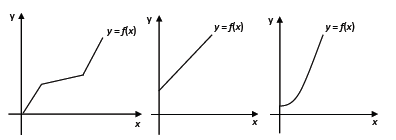
\includegraphics[width=6cm,height=3cm]{naikturun1.png}

Beberapa grafik fungsi naik dari kiri ke kanan

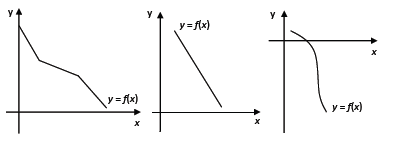
\includegraphics[width=6cm,height=3cm]{naikturun2.png}

Dari beberapa contoh grafik fungsi naik dan turun di atas,mari kita definisikan fungsi naik dan turun sebagai berikut.

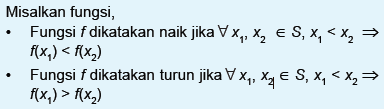
\includegraphics[width=10cm,height=3cm]{naikturun3.png}

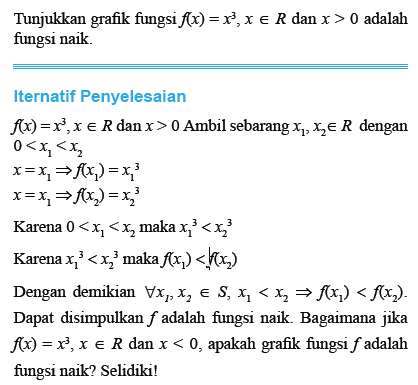
\includegraphics[width=10cm,height=7cm]{naikturun4.png}

\subsection{Aplikasi Turunan dalam Permasalahan Fungsi Naik dan Fungsi Turun}

Mari kita bahas aplikasi turunan dalam permasalahan fungsi naik dan fungsi turun dengan memperhatikan dan mengamati permasalahan berikut.\\

\textbf{Masalah 1}

Seorang nelayan melihat seekor lumba-lumba sedang berenang mengikuti kecepatan perahu mereka. Lumba-lumba tersebut berenang cepat, terkadang menyelam dan tiba-tiba melayang ke permukakaan air laut. Pada saat nelayan tersebut melihat lumba-lumba menyelam maka ia akan melihatnya melayang ke permukaan 15 detik kemudian dan kembali ke permukaan air laut setelah 3 detik di udara. Demikan pergerakan lumba-lumba tersebut diamati berperiode dalam beberapa interval waktu pengamatan.

Dari ilustrasi diatas, dapatkah kamu sketsa pergerakan lumba-lumba tersebut dalam 2 periode? Ingat pengertian periode pada pelajaran trigonometri di kelas X. Dapatkah kamu tentukan pada interval waktu berapakah lumbalumba tersebut bergerak naik atau turun? Dapatkah kamu temukan konsep fungsi naik/turun?\\

\textbf{Alternatif Penyelesaian:}

Sketsa pergerakan lumba-lumba dalam pengamatan tertentu

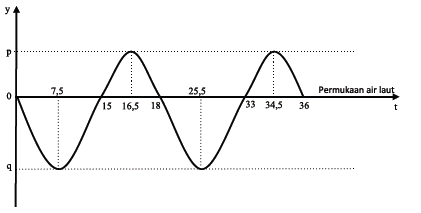
\includegraphics[width=12cm,height=5cm]{naikturun5.png}

Sketsa pergerakan naik/turun lumba-lumba dalam pengamatan tertentu

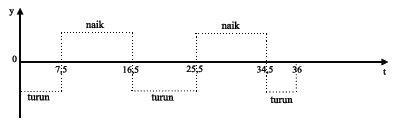
\includegraphics[width=12cm,height=5cm]{naikturun6.png}

Secara geometri pada sketsa di atas, lumba-lumba bergerak turun di interval 0 < t < 7,5 atau 16,5 < t < 25,5 atau 34,5 < t < 36 dan disebut bergerak naik di interval 7,5 < t < 16,5 atau 25,5 < t < 34,5.
%-------------Sesi 2---------------------------------
Coba kamu amati beberapa garis singgung yang menyinggung kurva di saat fungsi naik atau turun di bawah ini. Garis singgung 1 dan 3 menyinggung kurva pada saat fungsi naik dan garis singgung 2 dan 4 menyinggung kurva pada saat fungsi turun.

Garis singgung di interval fungsi naik/turun

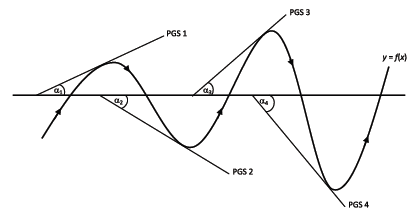
\includegraphics[width=14cm,height=7cm]{naikturun7.png}

Selanjutnya, mari kita bahas hubungan persamaan garis singgung dengan fungsi naik atau turun. Pada konsep
persamaan garis lurus, gradien garis adalah tangen sudut yang dibentuk oleh garis itu sendiri dengan sumbu x positif.Pada persamaan garis singgung, gradien adalah tangen sudut garis tersebut dengan sumbu positif sama dengan nilai turunan pertama di titik singgungnya. Pada gambar di atas, misalkan besar masing-masing sudut adalah 0 < $\propto $1 < 900 < $\propto $2 < 900 < $\propto $3 < 900 < $\propto $4 < 900 sehingga nilai
gradien atau tangen sudut setiap garis singgung ditunjukkan pada tabel berikut:

\begin{center}
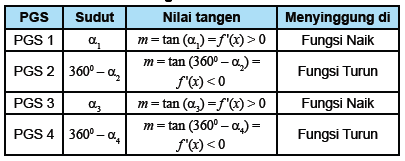
\includegraphics{naikturun8.png}
\end{center}

Coba kamu amati Gambar diatas dan Tabel sebelumnya Apakah kamu melihat konsep fungsi naik/turun. Coba kamu perhatikan kesimpulan berikut:

Jika garis singgung menyinggung di grafik fungsi naik maka garis singgung akan membentuk 

sudut terhadap sumbu x positif di kuadran I. Hal ini menyebabkan besar gradien adalah positif 

atau m = f '(x) > 0.

Jika garis singgung menyinggung di grafik fungsi turunmaka garis singgung akan membentuk 

sudut terhadap sumbu x positif di kuadran IV. Hal ini menyebabkan besar gradien adalah negatif 

atau m = f '(x) < 0.

Dengan demikian, dapat kita simpulkan bahwa fungsi f(x) yang dapat diturunkan pada interval I, akan mempunyai kondisi sebagai berikut:

\begin{center}
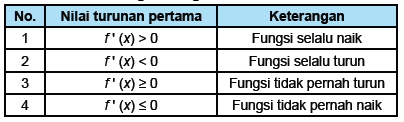
\includegraphics{naikturun9.png}
\end{center}

Misalkan f adalah fungsi bernilai real dan dapat
diturunkan pada setiap x $\in $I maka

1. Jika f '(x) > 0 maka fungsi selalu naik pada interval I.

2. Jika f '(x) < 0 maka fungsi selalu turun pada interval I.

3. Jika f '(x) $\geqslant $0 maka fungsi tidak pernah turun pada interval I.

4. Jika f '(x) $\leqslant $0 maka fungsi tidak pernah naik pada interval I.

Konsep di atas dapat digunakan jika kita sudah memiliki fungsi yang akan dianalisis. Tetapi banyak kasus seharihari harus dimodelkan terlebih dahulu sebelum dianalisis. Perhatikan kembali permasalahan berikut!\\

\textbf{Masalah:}

Tiga orang anak sedang berlomba melempar buah mangga di ketinggian 10 meter. Mereka berbaris menghadap pohon mangga sejauh 5 meter. Anak pertama akan melempar buah mangga tersebut kemudian akan dilanjutkan dengan anak kedua bila tidak mengenai sasaran. Lintasan lemparan setiap anak membentuk kurva parabola. Lemparan anak pertama mencapai ketinggian 9 meter dan batu jatuh 12 meter dari mereka. Lemparan anak kedua melintas di atas sasaran setinggi 5 meter. Anak ketiga berhasil mengenai sasaran. Tentu saja pemenangnya anak ketiga, bukan?
\\

\textbf{Permasalahan!}

Dapatkah kamu mensketsa lintasan lemparan ketiga anak tersebut? Dapatkah kamu membuat model matematika lintasan lemparan? Dapatkah kamu menentukan interval jarak agar masing-masing lemparan naik atau turun berdasarkan konsep turunan?\\


\textbf{Alternatif Penyelesaian}

\textbf{a. Sketsa Lintasan Lemparan}

Permasalahan di atas dapat kita analisis setelah kita modelkan fungsinya. Misalkan posisi awal mereka melempar adalah posisi titik asal O(0,0) pada koordinat kartesius, sehingga sketsa permasalahan di atas adalah sebagai berikut.

\begin{center}
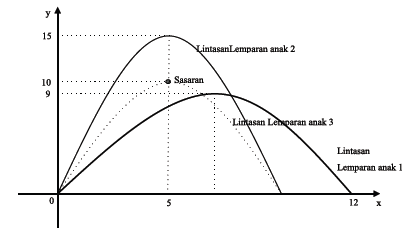
\includegraphics{naikturun10.png}
\end{center}

\textbf{b. Model Lintasan Lemparan}

Kamu masih ingat konsep fungsi kuadrat, bukan? Ingat
kembali konsep fungsi kuadrat yang melalui titik puncak
P($x_{p}, y_{p}) $dan titik sembarang P(x, y) adalah y – $y_{p} = a(x
$– $x_{p})^2 $sementara fungsi kuadrat yang melalui akar-akar x1,
x2 dan titik sembarang P(x, y) adalah y = a(x – $x_{1})(x $– $x_{2}),
$dengan $x_{p}= \dfrac{x_{1}-x_{2}}{2}
$dan a $\neq $0, a bilangan real. Jadi, model
lintasan lemparan setiap anak tersebut adalah:

\textbf{Lintasan lemparan anak pertama}

Lintasan melalui titik O(0,0) dan puncak $p_{1}$(6,9).

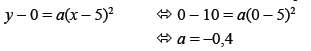
\includegraphics{naikturun11.png}

Fungsi lintasan lemparan anak pertama adalah y = –0,25$x^{2} $+ 3x.\\

\textbf{Lintasan lemparan anak kedua}

Lintasan melalui titik O(0,0) dan puncak $P_{2}$(5,15).

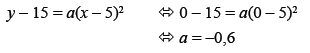
\includegraphics{naikturun12.png}

Fungsi lintasan lemparan anak kedua adalah y = –0,6$x^{2} $+ 6x.\\

\textbf{Lintasan lemparan anak ketiga}

Lintasan melalui titik O(0,0) dan puncak P3(5,10).

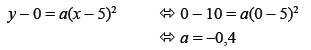
\includegraphics{naikturun13.png}

Fungsi lintasan lemparan anak ketiga adalah y = –0,4x2 +
4x.\\

\textbf{c. Interval Fungsi Naik/Turun Fungsi Lintasan}

Coba kamu amati kembali Gambar seketsa lintasan lemparan Secara geometri,jelas kita lihat interval fungsi naik/turun pada masingmasing lintasan, seperti pada tabel berikut:\\

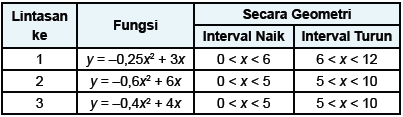
\includegraphics{naikturun14.png}\\

Mari kita tunjukkan kembali interval fungsi naik/turun dengan meng-gunakan konsep turunan yang telah kita pelajari sebelumnya.\\

\textbf{Fungsi naik/turun pada lintasan lemparan anak 1}

Fungsi yang telah diperoleh adalah y = –0,25$x^{2} $+ 3x sehingga y = –0,5$x^{2} $+ 3x. Jadi,

fungsi akan naik: y = –0,5$x^{2} $+ 3x$ \Leftrightarrow $x < 6

fungsi akan turun: y = –0,5x + 3 < 0$ \Leftrightarrow $x > 6

Menurut ilustrasi, batu dilempar dari posisi awal O(0,0) dan jatuh pada posisi akhir Q(12,0) sehingga lintasan lemparan akan naik pada 0 < x < 6 dan turun pada 6 < x < 12.

Bagaimana menunjukkan interval fungsi naik/turun
dengan konsep turunan pada fungsi lintasan lemparan
anak 2 dan anak 3 diserahkan kepadamu.

\textbf {Contoh Soal:} 
Tentukanlah interval fungsi naik/turun fungsi f(x) = $x^{4} $– 2x$^{2}$

\textbf{Alternatif Penyelesaian}

Berdasarkan konsep, sebuah fungsi akan naik jika f '(x) > 0 sehingga:

f '(x) = 4x$^{3} $– 4x > 0$ \Leftrightarrow $4x(x – 1)(x + 1) > 0$ \Leftrightarrow $x = 0 atau x = 1 atau x = –1

Dengan menggunakan interval.

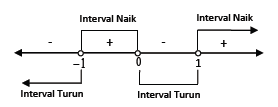
\includegraphics{naikturun15.png}\\

Jadi, kurva fungsi tersebut akan naik pada interval l –1 < x < 0 atau x > 1 tetapi turun pada interval x < –1 atau 0 < x < 1. Perhatikan sketsa kurva f(x) = x$^{4} $– 2x$^{2} $tersebut.\\

\begin{center}
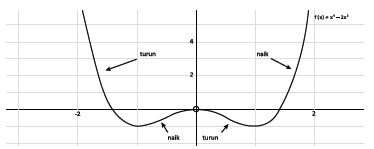
\includegraphics{naikturun16.png}\\
Gambar Fungsi naik/turun kurva f(x) = x4 – 2x2
\end{center}

\subsection{Aplikasi Konsep Turunan dalam
Permasalahan Maksimum dan Minimum}

Setelah menemukan konsep fungsi naik dan turun,
kita akan melanjutkan pembelajaran ke permasalahan
maksimum dan minimum serta titik belok suatu fungsi.
Tentu saja, kita masih melakukan pengamatan terhadap
garis singgung kurva. Aplikasi yang akan dibahas adalah permasalahan titik optimal fungsi dalam interval terbuka dan tertutup, titik belok, dan permasalahan kecepatan maupun percepatan.\\

\textbf{1.Menemukan konsep maksimum dan minimum di interval terbuka}

\textbf{Masalah: }
Seorang anak menarik sebuah tali yang cukup
panjang. Kemudian dia membuat gelombang dari
tali dengan menghentakkan tali tersebut ke atas dan
ke bawah sehingga terbentuk sebuah gelombang
berjalan. Dia terus mengamati gelombang tali yang
dia buat. Dia melihat bahwa gelombang tali memiliki
puncak maksimum maupun minimum. Dapatkah
kamu menemukan konsep nilai maksimum ataupun
minimum dari sebuah fungsi?

\textbf{Penyelesaian :}
Gradien garis singgung adalah tangen sudut yang
dibentuk oleh garis itu sendiri dengan sumbu x positif atau turunan pertama dari titik singgungnya.

\begin{center}
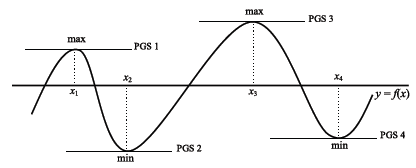
\includegraphics{naikturun17.png}\\
Gambar Sketsa gelombang tali
\end{center}

Coba kamu amati gambar di atas. Garis singgung
(PGS 1, PGS 2, PGS 3 dan PGS 4) adalah garis horizontal atau y = c, c konstan, sehingga gradiennya
adalah m = 0. Keempat garis singgung tersebut menyinggung kurva di titik puncak/optimal, di absis x =$ x_{1}, x = x_{2}, x = x_{3}, dan x = x_{4}$. Dari pengamatan, dapat disimpulkan bahwa sebuah fungsi akan mencapai optimal(maksimum/minimum) pada suatu daerah jika m = f '(x) = 0. Titik yang memenuhi f '(x) = 0 disebut titik stasioner. Berikutnya, kita akan mencoba menemukan hubungan antara titik stasioner dengan turunan kedua fungsi. Pada Gambar sketsa gelombang tali, f '$(x_{1}) = 0, f '(x_{2}) = 0, f '(x_{3}) = 0 dan f '(x_{4}) $= 0. Artinya kurva turunan pertama fungsi melalui sumbu x di titik A($x_{1}, 0), B(x_{2}, 0), C(x_{3}, 0) dan D(x_{4}$, 0).

Coba kamu amati kurva turunan pertama fungsi dan
garis singgungnya sebagai berikut. Kesimpulan apa
yang kamu dapat berikan?

\begin{center}
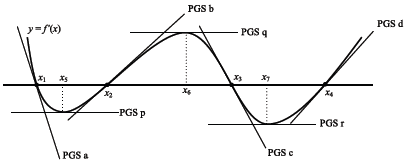
\includegraphics{naikturun18.png}\\
Gambar Hubungan garis singgung kurva m = f '(x)
dengan titik stasioner
\end{center}

Titik A($x_{1}, y_{1})$ adalah titik maksimum pada Gambar sketsa gelombang tali sehingga titik dengan absis x = x1 adalah titik stasioner karena f '($x_{1})$ = 0. Per-samaan garis singgung kurva dengan gradien M pada fungsi m = f '(x) menyinggung di titik x = $x_{1}$ membentuk sudut di kuadran IV sehingga nilai tangen sudut bernilai negatif. Hal ini mengakibatkan M = m ' = f ''$(x_{1}) $< 0. Dengan kata lain, titik A($x_{1}, y_{1})$ adalah titik maksimum jika f '$(x_{1}) = 0 dan f "(x_{1}$) < 0.

Kesimpulan: Lihat Gambar hubungan garis singgung kurva, misalkan gradien persamaan garis singgung kurva m = f '(x) adalah M sehingga M = m ' = f ''(x) maka hubungan turunan kedua dengan titik stasioner adalah:

\begin{center}
\includegraphics{naikturun19.png}\\
Tabel Hubungan turunan kedua fungsi dengan
titik optimal (stasioner)
\end{center}

\textbf{Sifat:}Misalkan f adalah fungsi bernilai real yang kontinu
dan memiliki turunan pertama dan kedua pada $x_{1} \in I$
sehingga:

1. Jika f '$(x_{1}) = 0 maka titik (x_{1}, f(x_{1}))$disebut stasioner/
kritis

2. Jika f '$(x_{1}) = 0 dan f "(x_{1}) > 0 maka titk (x1, f(x_{1}))$disebut titik balik minimum fungsi

3. Jika f '$(x_{1}) = 0 dan f "(x_{1}) < 0 maka titik (x1, f(x_{1}))$disebut titik balik maksimum fungsi

4. Jika f ''$(x_{1}) = 0 maka titik (x_{1}, f(x_{1})) $disebut titik belok\\

\textbf{Contoh Soal:}Tentukanlah titik balik fungsi kuadrat f(x) = $x^{2} $– 4x + 3

\textbf{Penyelesaian 1 (Berdasarkan Konsep
Fungsi Kuadrat)}

Dengan mengingat kembali pelajaran fungsi kuadrat.
Sebuah fungsi f(x) = $ax^{2} $+ bx + c mempunyai titik balik B(-$\dfrac{b}{2a}$,-$\dfrac{D}{4a}$) dimana fungsi mencapai maksimum untuk a < 0 dan mencapai minimum untuk a > 0 sehingga fungsi
f(x) = $x^{2}$ – 4x + 3 mempunyai titik balik minimum pada B(-$\dfrac{-4}{2(1)}$,-$\dfrac{(-4)^{2}-4(1)(3)}{4(1)}$=B(2,-1).\\

\textbf{Penyelesaian 2 (Berdasarkan Konsep
Turunan)}

Dengan menggunakan konsep turunan di atas maka
fungsi f(x) = $x^{2} $– 4x + 3 mempunyai stasioner: f '(x) = 2x – 4 = 0 atau x = 2 dan dengan mensubstitusi nilai x = 2 ke fungsi y = f(x) = $x^{2} $– 4x + 3 diperoleh y = –1 sehingga titik stasioner adalah B(2, –1). Mari kita periksa jenis keoptimalan fungsi tersebut dengan melihat nilai turunan keduanya pada titik tersebut. f "(x) = 2 atau f "(2) = 2 > 0.
Berdasarkan konsep, titik tersebut adalah titik minimum. Jadi, titik balik fungsi kuadrat f(x) = $x^{2} $– 4x + 3 adalah minimum di B(2, –1).

\begin{center}
\includegraphics{naikturun20.png}\\
Gambar Titik balik fungsi kuadrat f(x) = $x^{2}$ – 4x + 3
\end{center}

\section{Persamaan Garis Singgung dan Garis Normal}\index{Persamaan Garis Singgung dan Garis Normal}
%----------------------------------------------------------------------------------------
%	CHAPTER 9
%----------------------------------------------------------------------------------------

\chapterimage{chapter_head_2.pdf} % Chapter heading image

\chapter{Integral Tak Tentu Fungsi Aljabar}

\section{Pengertian Integral Tak Tentu Fungsi Aljabar}\index{Pengertian Integral Tak Tentu Fungsi Aljabar}

\section{Sifat-Sifat Integral Tak Tentu Fungsi Aljabar}\index{Sifat-Sifat Integral Tak Tentu Fungsi Aljabar}

\section{Penerapan Integral Tak Tentu Fungsi Aljabar}\index{Penerapan Integral Tak Tentu Fungsi Aljabar}


%----------------------------------------------------------------------------------------

%	BIBLIOGRAPHY
%----------------------------------------------------------------------------------------

\chapter*{Bibliography}
\addcontentsline{toc}{chapter}{\textcolor{ocre}{Bibliography}}
\section*{Books}
\addcontentsline{toc}{section}{Books}
\printbibliography[heading=bibempty,type=book]
\section*{Articles}
\addcontentsline{toc}{section}{Articles}
\printbibliography[heading=bibempty,type=article]

%----------------------------------------------------------------------------------------
%	INDEX
%----------------------------------------------------------------------------------------

\cleardoublepage
\phantomsection
\setlength{\columnsep}{0.75cm}
\addcontentsline{toc}{chapter}{\textcolor{ocre}{Index}}
\printindex

%----------------------------------------------------------------------------------------

\end{document}
